
\documentclass[preprint,12pt]{elsarticle}

\usepackage[T1]{fontenc}
\usepackage{lmodern}
\usepackage{amsmath,amssymb}
\usepackage{booktabs,array,graphicx,xcolor,tabularx}
\usepackage{microtype}
\usepackage{xspace}
\usepackage{tikz}
\usetikzlibrary{positioning,arrows.meta,fit,calc}
\usepackage[hidelinks]{hyperref}
\usepackage{url}
\Urlmuskip=0mu plus 2mu\relax
\def\UrlBreaks{\do\/\do\-\do\.}
\usepackage[capitalise,nameinlink]{cleveref}
\usepackage{caption}
\usepackage[section]{placeins}
\captionsetup{font=small,labelfont=bf}
\setlength{\emergencystretch}{2em}
\renewcommand{\topfraction}{0.9}\renewcommand{\textfraction}{0.08}\renewcommand{\floatpagefraction}{0.7}

\newcommand{\ms}{\,ms\xspace}
\newcommand{\KiB}{\,KiB\xspace}
\newcommand{\Mbits}{\,Mbit/s\xspace}
\newcommand{\cpu}{\mathrm{cpu}}

\journal{Computers \& Security}
\hypersetup{pdfauthor={Trong-Hieu Dinh, Trong-Minh Hoang}}

\begin{document}
\begin{frontmatter}

\title{Predicting the Transport Cost of Post-Quantum Authentication in Financial Messaging}

\author[1]{Trong-Hieu DINH\fnref{orc1}}\ead{hieudt@hvnh.edu.vn}
\author[2]{Trong-Minh HOANG\corref{cor1}\fnref{orc2}}\ead{hoangtrongminh@ptit.edu.vn}
\fntext[orc1]{ORCID: \href{https://orcid.org/0009-0005-0601-3229}{0009-0005-0601-3229}}
\fntext[orc2]{ORCID: \href{https://orcid.org/0000-0001-8486-2940}{0000-0001-8486-2940}}

\cortext[cor1]{Corresponding author: Trong-Minh HOANG}

\affiliation[1]{organization={Banking Academy of Vietnam}, city={Hanoi}, country={Vietnam}}
\affiliation[2]{organization={Posts and Telecommunications Institute of Technology}, city={Hanoi}, country={Vietnam}}

\begin{abstract}
Post-quantum signatures are one to two orders of magnitude larger than their classical counterparts and enlarge the certificate chains and signed objects of mutual Transport Layer Security (mTLS) payment transactions. Their cost is paid mainly in round trips: a flight that exceeds the Transmission Control Protocol (TCP) congestion window waits one more round-trip time (RTT), and message size alone does not tell which flight does. We propose a per-segment transport model that locates these thresholds from two observed behaviors of the tested stack, the OpenSSL write pattern and the Linux slow-start window validation. On 226 kernel-emulated configurations (6\,960 transactions), the model predicts excess latency with a mean absolute error (MAE) of 1.65\ms, against 4.70\ms and whole-round-trip errors for an idealized closed-form model. The 144 configurations measured later, which were not used to identify the mechanisms, give 2.04\ms, and a systematic residual of a few milliseconds remains. The validation covers ISO~8583-sized requests and one SWIFT-sized transaction; the other profiles and suites are model applications. Applied to thirteen cryptographic suites and six financial protocol profiles, the model shows that raising both ML-DSA-65 (Module-Lattice-Based Digital Signature Algorithm) chain depths from 1 to 4 in a SWIFT~MX transaction adds 60.0\ms at a 30\ms RTT, of which 56.5\ms is slow-start waiting, and that size-dependent transport overhead exceeds the modeled cryptographic-primitive time in 75.6\% of the equally weighted ML-DSA-65 cold-connection grid. Chain depth, certificate embedding and the initial window set post-quantum transaction latency on the tested stack.
\end{abstract}

\begin{highlights}
\item Linux window validation and OpenSSL writes set round-trip thresholds.
\item Excess-latency MAE is 1.65\ms over 226 configurations (idealized: 4.70\ms).
\item Later off-grid measurements give an MAE of 2.04\ms.
\item Mutual-TLS chains and application signatures jointly set the transport cost.
\end{highlights}

\begin{keyword}
post-quantum cryptography \sep financial messaging \sep mutual TLS \sep TCP congestion window \sep certificate chains \sep latency model
\end{keyword}
\end{frontmatter}

%% ============================================================================================
\section{Introduction}
\label{sec:intro}

A payment gateway that uses mutual Transport Layer Security (mTLS) exchanges two certificate chains at connection establishment and may sign each payment request and response. Migration to post-quantum authentication expands these objects at the transport and application layers. An ML-DSA-65 signature occupies 3\,309\,bytes~\cite{fips204}; an Elliptic Curve Digital Signature Algorithm (ECDSA) P-256 signature occupies at most 72\,bytes in DER encoding~\cite{fips186}. A flight is a group of messages that one endpoint sends before waiting for the peer. When a flight exceeds the available Transmission Control Protocol (TCP) congestion window, the sender waits for acknowledgments (ACKs), and the delay grows with the round-trip time (RTT).

The migration follows from the vulnerability of Rivest–Shamir–Adleman (RSA) and elliptic-curve cryptography to a sufficiently large quantum computer~\cite{shor1994}. For confidentiality, the migration schedule depends on the lifetime of recorded information~\cite{mosca2018,baradziej2026}. The National Institute of Standards and Technology (NIST) standardized the Module-Lattice-Based Key-Encapsulation Mechanism (ML-KEM), the Module-Lattice-Based Digital Signature Algorithm (ML-DSA) and the Stateless Hash-Based Digital Signature Algorithm (SLH-DSA) in 2024~\cite{fips203,fips204,fips205}. Studies in this journal assess the quantum risk to network protocols and infrastructure~\cite{baseri2024,baseri2026}, and central-bank pilots have demonstrated post-quantum tunnels and signed financial messages~\cite{bis_leap2023,bis_leap2025}. Selecting certificate chains and message-signing profiles requires predicting the transport cost of each authenticated transaction.

The dominant approach estimates this cost from object sizes and the initial congestion window. Three limitations remain. First, measurement studies report handshake slowdown for given certificate sizes and initial windows, and they do not predict which flight incurs an additional RTT on a specified implementation~\cite{sikeridis2020,paquin2020}. Evaluation frameworks for post-quantum TLS measure handshake throughput and bytes under controlled loss and delay~\cite{montenegro2026} but do not predict individual flights either. Second, size analyses compare flight bytes with the initial window expressed in bytes~\cite{kampanakis2022}. This comparison is equivalent to dividing the flight size by the maximum segment size (MSS) and rounding up. The tested OpenSSL library writes handshake data through a 4\,096-byte buffer, which also decides when the ServerHello leaves~\cite{sosnowski2023}, and the Linux kernel validates window growth before enlarging the window~\cite{linuxtcp}. No earlier study uses these two behaviors to predict which flights cross the window. Each mechanism changes the segment count or the window available to the next flight. Finally, financial-system pilots measure tunnel setup and message signing but do not decompose the transport cost of mTLS chains and application signatures~\cite{bis_leap2023,bis_leap2025}. Extensible Markup Language Signature (XMLDSig), JSON Web Signature (JWS) and Demonstrating Proof of Possession (DPoP) objects add bytes above TLS.

This paper develops a model that links authentication objects to library writes and TCP waiting. The scope is one Linux/OpenSSL stack on a wired link. The financial content of the model lies in the objects it carries: the certificate chains of the two mTLS peers and the application-layer signatures of the payment protocols. Linux/OpenSSL is an open, measurable choice of transport; we have no evidence that a particular bank gateway runs on it, and the write pattern of the library and the window rule of the kernel are replaceable inputs of the model. The study makes three contributions.
\begin{itemize}
\item Method: we incorporate two observed stack mechanisms, the OpenSSL write pattern and Linux-style slow-start window validation, into a per-segment transport model.
\item Implementation: we apply the model to thirteen suites and six financial and application programming interface (API) profiles. Each profile carries the certificate chains of the two mTLS peers and its application-layer signatures. The latency decomposition separates serialization, propagation, slow-start waiting, and cryptographic computation.
\item Evaluation: we compare the model with real OpenSSL transactions on 226 configurations. The mean absolute error (MAE) of configuration-level excess latency is 1.65\ms; the idealized closed-form model gives 4.70\ms. We quantify the effect of chain depth, certificate embedding, connection reuse and certificate compression, and report the sensitivity of each effect to the initial window and to the assumed processing cost.
\end{itemize}

The empirical evidence comes from synthetic bank-like certificates and request-response probes on a kernel-emulated wired link. The protocol sweep is a model application. It does not represent measured bank traffic or backend payment processing. Measurements of one TCP proxy define the tested middlebox case. Larger middlebox delays are hypothetical sensitivity inputs. \Cref{sec:related} reviews prior work. \Cref{sec:method} defines the model and its inputs. \Cref{sec:testbed} presents the transport mechanisms and the experimental validation. \Cref{sec:results} reports the protocol-level predictions. \Cref{sec:discussion} discusses deployment implications and limitations, and \cref{sec:conclusion} concludes the paper.

\section{Related work}
\label{sec:related}
\Cref{tab:related} lists the closest studies by setting and evidence. The columns record whether a study varies the network condition (Net.), the transmitted certificate-chain depth (Depth) and the application signatures (Fin.\ msgs), and whether it provides a predictive transport model (Model). IKEv2/IPsec denotes Internet Key Exchange version~2 over Internet Protocol Security, DTLS denotes Datagram TLS, and BdF-MAS denotes the Banque de France-Monetary Authority of Singapore trial. ``Not reported'' marks missing information, and ``n/a'' marks inapplicable information. The studies fall into three technical directions.

\begin{table}[tp]
\centering\footnotesize
\caption{Related studies and evaluated components.}
\label{tab:related}
\renewcommand{\arraystretch}{1.0}\setlength{\tabcolsep}{3pt}
\begin{tabularx}{\textwidth}{@{}>{\raggedright\arraybackslash}p{0.14\textwidth}>{\raggedright\arraybackslash}X>{\raggedright\arraybackslash}p{0.14\textwidth}>{\raggedright\arraybackslash}p{0.13\textwidth}>{\raggedright\arraybackslash}p{0.14\textwidth}>{\raggedright\arraybackslash}p{0.075\textwidth}@{}}
\toprule
Study & Setting and method & Net. & Depth & Fin.\ msgs & Model \\
\midrule
Sikeridis et al.~\cite{sikeridis2020} & TLS~1.3, local client to cloud server & real Internet path; initial window & 1--2 intermediates; mixed-algorithm chains & no & no \\
Paquin et al.~\cite{paquin2020} & TLS, Linux-emulated network & 4 latencies, loss 0--20\% & root to server only & no & no \\
Raavi et al.~\cite{raavi2025} & TLS~1.3/TCP packet capture, local virtual machines & none (local) & single certificate, not varied & no & no \\
Sosnowski et al.~\cite{sosnowski2023} & Sequential TLS~1.3 handshakes, two hosts, hardware timestamps, CPU profiling & loss, delay, bandwidth limits & not reported & no & no \\
Westerbaan \cite{westerbaan2021} & Field experiment, about $10^6$ live connections & real clients worldwide; initial window 30 & chain size, via dummy 1\,KiB certificates & no & no \\
Kampanakis and Kallitsis \cite{kampanakis2022} & Size analysis, (D)TLS and QUIC & QUIC amplification limit & 1--4 intermediates; suppression & no & no \\
Project Leap~\cite{bis_leap2023} & IKEv2/IPsec tunnels between two central banks, 100 runs per combination & public network, not varied & not reported & pacs.008 as payload only & no \\
Project Leap Phase 2~\cite{bis_leap2025} & T2 test environment, liquidity transfers; receiver-side verification time & not reported & none (raw keys, no certificates) & ISO~20022 header signature (Dilithium) & no \\
BdF--MAS~\cite{bdfmas2024} & Hybrid e-mail across continents & real Internet & n/a & e-mail signatures & no \\
\midrule
\textbf{This work} & Model validated on real OpenSSL~3.5 handshakes, signed objects and transactions over an emulated link & RTT, bit rate, MTU, window, middlebox delay & 1--4 & ISO~8583, ISO~20022, SWIFT~MX, FAPI~2.0 & yes \\
\bottomrule
\end{tabularx}
\end{table}

\paragraph{Authentication size and transport thresholds}
This direction measures how authentication size affects handshake latency. Early work established that the size of post-quantum certificates, not the computation, is the practical obstacle. Kampanakis et~al.\ analyzed how post-quantum X.509 certificates are fragmented in TLS and IKEv2 and tested the analysis experimentally~\cite{kampanakis2018}. Sikeridis et~al.\ measured TLS~1.3 with several signature candidates and certificate-chain compositions~\cite{sikeridis2020}. Their TLS and Secure Shell (SSH) study showed that a larger initial window reduces the post-quantum slowdown~\cite{sikeridis2020b}. Paquin et~al.\ evaluated latency and packet loss on a Linux-emulated network~\cite{paquin2020}. B{\"u}rstinghaus-Steinbach et~al.\ showed that hash-based signatures are costly on embedded servers~\cite{burstinghaus2020}. Raavi et~al.\ captured the TCP packetization of post-quantum TLS handshakes with a single certificate on local virtual machines~\cite{raavi2025}. Montenegro et~al.\ built a containerized OpenSSL framework and counted TLS handshakes per 10\,s and bytes per handshake for classical, hybrid and post-quantum key exchange and signatures, with mutual authentication, delays of 1, 10 and 100\ms and packet loss of 0.1--1\%; their certificate chain has two certificates of one algorithm, and other chain depths are left to future work~\cite{montenegro2026}. These studies establish the effect of authentication size, network conditions, and window settings. Sosnowski et~al.\ combined black- and white-box measurements of post-quantum TLS~1.3 under emulated loss, bandwidth and delay~\cite{sosnowski2023}. They observed that the internal buffer of OpenSSL decides when the ServerHello leaves, but did not use this to predict segments or round trips. These studies take byte counts, packet captures, and end-to-end times as the unit of analysis, with fixed or single-level chains. No study combines the write pattern of the TLS library with kernel window growth to predict which flight crosses a window threshold on a specified implementation, and validates the prediction against real transactions.

\paragraph{Certificate reduction}
This direction reduces authentication traffic. Field measurements with enlarged certificate chains show that the initial window sets the handshake slowdown and that some clients or middleboxes fail at large handshake sizes~\cite{westerbaan2021}. Suppression of intermediate certificates reduces authentication bytes~\cite{kampanakis2022}. Key-based authentication replaces handshake signatures~\cite{schwabe2020}, and Merkle Tree Certificates replace per-certificate signatures with inclusion proofs~\cite{mtcdraft}. These approaches assume that fewer bytes yield lower latency. A byte reduction removes an RTT only when it moves a flight below a transport threshold. The locations of these thresholds for certificate-based TLS and application objects remain open.

\paragraph{Financial-system deployments}
This direction tests post-quantum cryptography in operational financial settings. Project Leap Phase~1 measured post-quantum IPsec tunnel establishment between central banks~\cite{bis_leap2023}. Project Leap Phase~2 evaluated post-quantum signing of ISO~20022 messages in a payment-system test environment with software keys and raw public keys. It reported receiver-side verification times of 209.9\ms for round-3 Dilithium category~3 and 28.1\ms for RSA~\cite{bis_leap2025}. The Banque de France trial deployed a post-quantum IPsec VPN with hardware security modules and Dilithium certificates, focused on interoperability and crypto-agility, and reported tunnel set-up times of 4 to 5\,s with FrodoKEM level~5 and the module; the report says that this result would have to be re-examined for a TLS connection~\cite{bdf2022}. The BdF-MAS trial demonstrated hybrid signed and encrypted e-mail between two central banks~\cite{bdfmas2024}. Surveys of quantum-safe network protocols and infrastructure identify migration and interoperability risk~\cite{baseri2024,baseri2026}. Supervisory and regulatory work frames the migration as a matter of planning, cryptographic inventory, and operational resilience~\cite{g7qtwg2026,andriani2024,dora2022,janciute2025}. These studies take integration, tunnel setup, and risk, or governance as the object of analysis. None of them measures certificate chains at more than one depth, and none of them decomposes the transport cost of mTLS chains and application signatures in payment protocols. This decomposition is the gap that the present study addresses.

\paragraph{Scope of the contribution}
Prior work establishes that larger authentication objects incur additional RTTs. This study contributes an implementation-specific predictive model, its empirical evaluation, and the interaction of mTLS chains and application signatures in representative financial profiles. It introduces no cryptographic primitive and no security proof.

\section{System model and measurement inputs}
\label{sec:method}

A transaction between a payment client and a gateway consists of a TCP connection, a TLS~1.3 handshake, and one or more request-response exchanges. The model predicts its latency from the authentication objects and the link parameters. \Cref{fig:pipeline} summarizes the pipeline. A flow builder converts a suite, a protocol profile, a chain depth, $d$, and a connection mode into an ordered sequence of central processing unit (CPU) steps and byte transfers. A cold transaction opens a new TCP and TLS connection; a warm transaction reuses an established connection. A replay engine executes the flow over a wired link. In \cref{fig:pipeline}, $\pi$ and $\theta$ denote the optional middlebox delay and its segment threshold (\cref{sec:transport}), and DER denotes the Distinguished Encoding Rules. \Cref{tab:protocols,tab:constants} in \ref{app:inputs} list the parameters, and the code and data are public (see Data availability).

\begin{figure}[t]
\centering
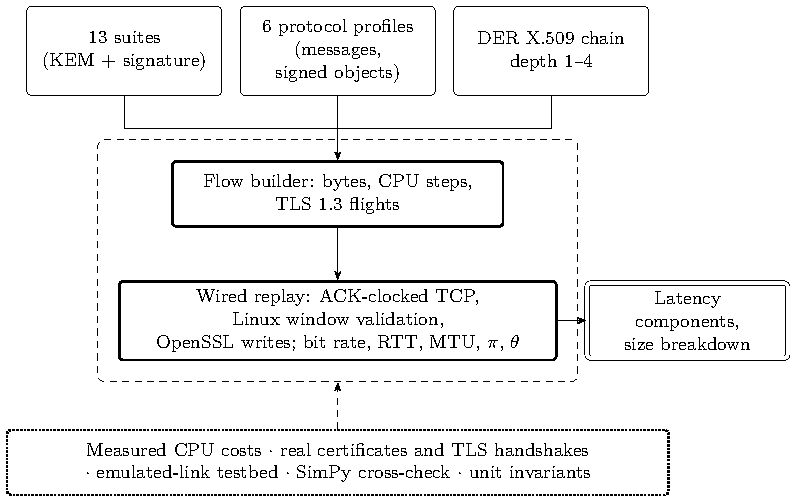
\includegraphics[width=\textwidth]{figures/fig_pipeline}
\caption{Model pipeline and measurement inputs.}
\label{fig:pipeline}
\end{figure}

\subsection{Cryptographic suites and protocol profiles}
A suite pairs a key-establishment mechanism, a key exchange or a key-encapsulation mechanism (KEM), with one signature scheme. The signature scheme signs the certificate chain, the TLS \texttt{CertificateVerify} message and the application objects. \Cref{tab:algos} gives the public-key (PK), SubjectPublicKeyInfo (SPKI) and signature sizes in bytes and the median times on one Cortex-X925 core with OpenSSL~3.5.4 (liboqs~0.14.0 for Falcon). Its key-establishment rows give the TLS key-share sizes and the client and server computation. The classical baseline is ECDSA-P256 with the X25519 elliptic-curve Diffie--Hellman function. The classical suites add RSA-2048 and RSA-3072 with Elliptic Curve Diffie--Hellman Ephemeral (ECDHE) key exchange. ECDSA-P256 with the hybrid X25519MLKEM768 key share migrates key establishment only. The post-quantum suites pair ML-KEM with ML-DSA-44/65/87, with Falcon-512/1024~\cite{falcon2020} or with SLH-DSA-128s/128f. The composite suites use ML-DSA-44/65 + ECDSA-P256 certificates~\cite{compositedraft} with the hybrid key share of RFC~10024~\cite{hybriddraft}. The composite specification was an Internet-Draft in the RFC Editor queue at the time of writing. Sizes follow the cited specifications. The suites span different NIST security categories. Their performance ranking is not an equal-security comparison. Composite sizes and CPU costs are the sums of the constituent schemes; we did not measure interoperable composite objects. CPU costs are measured (\cref{sec:meas}). The sweeps scale them by 2 (the measured efficiency core), by 4 (close to the measured x86 core) and by 16 (an assumed slow-processing case). The factor 16 is not an HSM measurement.

The six profiles are ISO~8583 0200/0210 card messages protected by symmetric message authentication codes (MACs)~\cite{iso8583}; ISO~20022 pacs.008/pacs.002 payment messages~\cite{iso20022} and SWIFT~MX messages, each signed with XMLDSig~\cite{xmldsig} over mTLS; OAuth~2.0 with bearer tokens~\cite{rfc6749,rfc6750}; OpenID Connect (OIDC)~\cite{oidccore}; and Financial-grade API (FAPI)~2.0~\cite{fapi2} with signed request objects, DPoP~\cite{rfc9449} and mTLS~\cite{rfc8705}. SWIFT~MX denotes the ISO~20022-based message format of the Society for Worldwide Interbank Financial Telecommunication (SWIFT). The profiles are representative scenario choices. They are not mandatory combinations of security mechanisms. The selected FAPI profile combines DPoP and mTLS. The XMLDSig profiles embed the signer certificate by default. Message sizes exclude algorithm-dependent bytes. The model adds encoded signatures, embedded public keys and signer certificates according to each profile. \Cref{sec:sens} evaluates a reference to the XML signer certificate in place of embedding.

\begin{table}[t]
\centering\small
\caption{Cryptographic inputs.}
\label{tab:algos}
\resizebox{\textwidth}{!}{\begin{tabular}{@{}llrrrrrr@{}}
\toprule
Signature & Family & PK & SPKI & Sig. & Sign & Verify & Pair \\
 & & (B) & (B) & (B) & (ms) & (ms) & KEM \\
\midrule
RSA-2048 & classical & 270 & 294 & 256 & 0.491 & 0.0147 & ECDHE-P256 \\
RSA-3072 & classical & 398 & 422 & 384 & 1.451 & 0.0293 & ECDHE-P256 \\
ECDSA-P256 & classical & 65 & 91 & 72 & 0.01446 & 0.04112 & X25519 / hybrid \\
ML-DSA-44 & lattice & 1\,312 & 1\,334 & 2\,420 & 0.3594 & 0.06804 & ML-KEM-768 \\
ML-DSA-65 & lattice & 1\,952 & 1\,974 & 3\,309 & 0.586 & 0.103 & ML-KEM-768 \\
ML-DSA-87 & lattice & 2\,592 & 2\,614 & 4\,627 & 0.6691 & 0.1589 & ML-KEM-1024 \\
Falcon-512 & lattice & 897 & 919 & 666 & 0.1045 & 0.01755 & ML-KEM-768 \\
Falcon-1024 & lattice & 1\,793 & 1\,815 & 1\,280 & 0.2114 & 0.03098 & ML-KEM-1024 \\
SLH-DSA-128s & hash & 32 & 54 & 7\,856 & 170.8 & 0.1614 & ML-KEM-768 \\
SLH-DSA-128f & hash & 32 & 54 & 17\,088 & 8.2 & 0.5058 & ML-KEM-768 \\
ML-DSA-44+ECDSA-P256 & composite & 1\,377 & 1\,399 & 2\,492 & 0.37386 & 0.10916 & X25519MLKEM768 \\
ML-DSA-65+ECDSA-P256 & composite & 2\,017 & 2\,039 & 3\,381 & 0.60046 & 0.14412 & X25519MLKEM768 \\
\midrule
\multicolumn{8}{l}{\textit{Key establishment: key-share bytes; last two columns = client / server computation (ms)}} \\
\quad ECDHE-P256 & classical & \multicolumn{2}{r}{client 65} & \multicolumn{2}{r}{server 65} & 0.04251 & 0.04251 \\
\quad X25519 & classical & \multicolumn{2}{r}{client 32} & \multicolumn{2}{r}{server 32} & 0.03596 & 0.03596 \\
\quad X25519MLKEM768 & hybrid & \multicolumn{2}{r}{client 1\,216} & \multicolumn{2}{r}{server 1\,120} & 0.06844 & 0.04516 \\
\quad ML-KEM-768 & post-quantum & \multicolumn{2}{r}{client 1\,184} & \multicolumn{2}{r}{server 1\,088} & 0.03248 & 0.009197 \\
\quad ML-KEM-1024 & post-quantum & \multicolumn{2}{r}{client 1\,568} & \multicolumn{2}{r}{server 1\,568} & 0.04562 & 0.01183 \\
\bottomrule
\end{tabular}}
\end{table}

\subsection{Authentication objects and transaction flow}
The size of a modeled certificate controls the bytes of each authentication flight. A certificate $i$ has length
\begin{equation}
L_i=m_i+b_\mathrm{SPKI}+b_\sigma+4,
\label{eq:cert}
\end{equation}
where $L_i$ is the encoded length in bytes, $m_i$ is the algorithm-independent metadata length, $b_\mathrm{SPKI}$ is the length of the SPKI field, $b_\sigma$ is the signature length and 4\,bytes is the outer DER framing. \Cref{eq:cert} separates fixed metadata from the algorithm-dependent key and signature fields. We set $m_i=900$\,bytes for a leaf and $m_i=520$\,bytes for a certification authority (CA) certificate (empirical choice; \cref{sec:sens} varies the two values). A transmitted chain of depth $d$ contains the leaf and $d-1$ intermediates and excludes the root~\cite{rfc5280}. Under mTLS, the same $d$ applies to the two endpoint chains in the main sweep; \cref{tab:asym} gives them separate depths. An increase of $d$ by one adds one transmitted intermediate at each endpoint.

A cold transaction opens a new TCP connection and performs a full TLS~1.3 handshake~\cite{rfc8446}. The ordered transfers are the ClientHello, the server authentication flight, the client authentication flight, a separately written first request and the remaining request--response exchanges. The model charges key establishment, handshake signatures, $d+1$ verification operations per authenticated chain (with \texttt{CertificateVerify}) and all application signatures. These CPU steps are serial on the modeled critical path. The model does not overlap certificate processing with the reception of the remaining flight bytes.

\subsection{Per-segment transport model and latency decomposition}
\label{sec:transport}
The reference path uses Internet Protocol version~6 (IPv6). The maximum transmission unit (MTU) and the MSS satisfy $\mathrm{MSS}=\mathrm{MTU}-60$\,bytes. Each direction maintains its own congestion window. The initial window is $c_0=10$ segments~\cite{rfc6928,rfc5681}. A warm transaction reuses TLS without a handshake. Its reference window restarts at $c_0$ and represents an idle connection. A sensitivity case retains a 64-segment window and represents a busy connection.

The ACK clock sets when each segment of a flight leaves the sender. Consider a flight of $N$ segments on a first-in, first-out (FIFO) link. The segment release time $r_k$, start time $s_k$, departure time $\ell_k$ and ACK return time $a_k$ follow
\begin{equation}
\begin{split}
r_k&=\begin{cases}0,& k<c,\\a_{\lfloor(k-c)/2\rfloor},&k\ge c,\end{cases}\\
s_k&=\max(\ell_{k-1},r_k),\quad
\ell_k=s_k+\tau_k,\quad a_k=\ell_k+\mathrm{RTT},
\end{split}
\label{eq:flight}
\end{equation}
where $k=0,\dots,N-1$ is the zero-based segment index, $c$ is the window at the start of the flight, $\tau_k$ is the serialization time of segment $k$ and $\ell_{-1}=0$. The floor operator $\lfloor\cdot\rfloor$ releases two queued segments per returned ACK in slow start. \Cref{eq:flight} controls the slow-start waiting inside a flight. The last byte arrives at $\ell_{N-1}+\mathrm{RTT}/2$ under a symmetric one-way delay. The recurrence costs $\mathcal{O}(N)$ operations per flight. The model excludes ACK serialization, receive-window limits, packet loss and queueing from other flows.

The implementation-specific model represents two observed behaviors. First, the tested OpenSSL configuration writes handshake data through a 4\,096-byte buffer and writes the application request separately. With \texttt{TCP\_NODELAY}, a partial segment at a write boundary leaves the sender when the window permits it. The model accounts for these boundaries and coalesces queued tails when the window is exhausted. Second, the model updates the next flight window using Linux-style slow-start validation. In the inspected kernel headers, \texttt{tcp\_is\_cwnd\_limited()} first accepts an explicitly window-limited sender. In slow start, it then tests whether \texttt{snd\_cwnd} is below twice \texttt{max\_packets\_out}, the tracked maximum of outstanding packets~\cite{linuxtcp}. This test uses the tracked maximum. It does not use the instantaneous number of packets in flight. The model tracks the peak number of outstanding segments during ACK replay and updates the window between flights using this value. A short flight that uses less than half of the available window does not enlarge it in this abstraction. The source inspection covers Linux~6.11 and 6.14. We empirically examined the behavior of the testbed kernel (Linux~7.0); \cref{sec:mech} reports a plain-TCP measurement of the window on this kernel. RFC~7661 specifies a related congestion-window validation method for rate-limited traffic~\cite{rfc7661}. The model follows the inspected Linux rule and does not implement RFC~7661.

The idealized closed-form model is the baseline of this study. It uses $\lceil\text{bytes}/\mathrm{MSS}\rceil$ segments per flight, where $\lceil\cdot\rceil$ is the ceiling operator, and it enlarges the window by the segment count after each flight. The implementation-specific model keeps the ACK-clock recurrence of \cref{eq:flight} within each flight. It abstracts the observed stack. It does not execute the complete Linux TCP state machine.

The model decomposes the latency of a transaction as
\begin{equation}
T=T_\cpu+T_\mathrm{ser}+T_\mathrm{prop}+T_\mathrm{ssw}+T_\mathrm{pen},
\label{eq:latency}
\end{equation}
where $T_\cpu$ is cryptographic computation, $T_\mathrm{ser}$ is serialization, $T_\mathrm{prop}$ is propagation, $T_\mathrm{ssw}$ is slow-start waiting and $T_\mathrm{pen}$ is an optional added middlebox delay. \Cref{eq:latency} is exact for the serial model. Real processing can overlap network reception. The size-dependent transport overhead is
\begin{equation}
O=T_\mathrm{ser}+T_\mathrm{ssw}+T_\mathrm{pen}.
\label{eq:overhead}
\end{equation}
\Cref{eq:overhead} excludes $T_\mathrm{prop}$, since propagation is common to the compared suites. The comparison of $O$ with $T_\cpu$ states whether a transaction is transport-bound or computation-bound.

The optional delay term is $T_\mathrm{pen}=\pi\,\bigl|\{f:N_f>\theta\}\bigr|$, where $N_f$ is the segment count of flight $f$, $|\cdot|$ denotes set cardinality, $\pi$ is the added delay in milliseconds and $\theta$ is the segment threshold. The term represents a hypothetical size-threshold delay. It is not a measured law of middlebox processing. The reference value is $\pi=0$; larger values are sensitivity inputs. Reported connection failures with large handshakes~\cite{westerbaan2021} motivate the examination of size-related constraints. They do not calibrate $\pi$, and the model does not represent connection failures. Size outputs use KiB ($1\,\mathrm{KiB}=1024$\,bytes). Bit rates use decimal Mbit/s.

For certificate compression~\cite{rfc8879}, the model treats keys and signatures as incompressible. The compression ratio of DER metadata is 0.68 for the first certificate and 0.52 for each subsequent certificate (calibrated on five public bank and payment chains). The assumed client decompression rates are 330, 33, 3.3 and 0.33\,MB/s. These rates are sensitivity inputs. They are not measurements of embedded clients.

\subsection{Parameter space and reported quantities}
The main sweep contains 140\,400 cold-connection rows and 35\,100 warm-connection rows, for a total of 175\,500 rows. The cold rows form the full factorial of thirteen suites, six profiles, four chain depths, six bit rates (10, 100, 200, 400, 800 and 1\,600\Mbits), five RTTs (5, 12, 30, 50 and 100\ms), three MTUs (1\,280, 1\,500 and 9\,000\,bytes) and five assumed delays $\pi\in\{0,3,6,12,24\}$\ms. Warm rows transmit no chain and have a single depth state. The threshold is $\theta=4$ segments; a separate sweep uses $\theta\in\{2,4,8,16\}$.

Unless stated otherwise, individual predictions use 100\Mbits, a 30\ms RTT, an MTU of 1\,500\,bytes, $\pi=0$ and a cold connection. The baseline suite is ECDSA-P256 with X25519. The share of transport-bound rows is
\begin{equation}
\phi=\frac{\bigl|\{j:O_j>T_{\cpu,j}\}\bigr|}{J},
\label{eq:share}
\end{equation}
where $j$ indexes the $J$ equally weighted cold rows of the selected grid. $\phi$ is a descriptive fraction of the chosen grid. It is not an estimate of the probability of bank traffic. The grid with all $\pi$ values includes hypothetical nonzero delays. \Cref{tab:protocols} lists the protocol reference depths and fixed object sizes.

\subsection{Measured inputs}
\label{sec:meas}
\paragraph{Primitive costs} The Arm primitive benchmarks and object-size measurements ran on an NVIDIA GX10 (10 Cortex-X925 and 10 Cortex-A725 cores; Linux~6.14). A C harness measured per-operation costs via the high-level envelope (EVP) interface of OpenSSL~3.5.4~\cite{openssl35}, which the OpenSSL TLS stack uses. It covers RSA with probabilistic signature scheme (RSA-PSS) padding, ECDSA, X25519, P-256, ML-KEM, ML-DSA and SLH-DSA-SHA2. liboqs~0.14.0~\cite{stebila2016} provided Falcon. Each value is the median of seven 0.5\,s runs pinned to one core. The minimum and maximum of the seven runs lie within 0.6\% of the median for the median operation and within 6\% for the noisiest operation, ML-DSA-87 signing (\cref{tab:cpu}). ML-DSA-65 signing costs 0.59\ms with OpenSSL and 0.27\ms with liboqs. The cost depends on the implementation. SLH-DSA-128s signing takes 171\ms. The efficiency core is 2.0 times slower than the performance core.

To anchor the CPU scale on a second architecture, we repeated the measurement on one core of an Intel Core i7-5600U (Broadwell, 2.5\,GHz, AVX2, turbo disabled). This machine hosts the testbed of \cref{sec:testbed}. Elliptic-curve and lattice operations are 2.2 to 4.4 times slower than on the X925 (median 3.15 for signatures and 3.87 for key establishment). This core is about 1.4 times slower than the Cortex-A725. RSA signing is 1.7 times slower. The hash-based SLH-DSA is about 8 times slower, since this core has no SHA instruction extensions (\cref{tab:cpux86}). Two measurements on different cores of an idle machine agree within 4\% for signatures. The CPU scale of 4 in the sweeps corresponds to a measured x86 core. The CPU scale of 16 is an assumed processing slowdown and not an HSM measurement.

\paragraph{Certificates and handshakes} We generated DER hierarchies with a root, 0--3 intermediates and server and client leaves with bank-like extensions for RSA, ECDSA, ML-DSA and SLH-DSA. We recorded 56 configurations of real TLS~1.3 handshakes with OpenSSL \texttt{s\_server}/\texttt{s\_client} (21 handshakes each, depth 1--4, with and without mTLS) through a loopback relay that counts the bytes of each flight. OpenSSL~3.5 has no TLS code points for SLH-DSA or Falcon. Certificates and CPU measurements cover these schemes.

\paragraph{Application objects} We produced real signed application objects with OpenSSL: JWS client assertions and access tokens, DPoP proofs with the key in the JSON Object Signing and Encryption (JOSE) header and an XMLDSig signature over a pacs.008 document with the signer certificate in \texttt{KeyInfo}. We compared each object with the model.

\subsection{Implementation verification and input checks}
The test suites check byte accounting, latency-component sums and selected monotonicity properties. An independently implemented SimPy discrete-event scheduler reproduces the transport outputs across 126\,360 flows with a maximum absolute latency difference of $1.3\times10^{-11}$\ms. This comparison verifies the consistency of two implementations of the same assumptions. It does not validate the assumptions against a physical network. The full event-driven grid uses the implementation-specific model; an additional 20\,000-flow sample checks the idealized model.

With certificate metadata calibrated on ECDSA, the predicted sizes of the generated certificates differ by at most 0.8\% for the measured RSA, ML-DSA and SLH-DSA certificates (\cref{tab:certs}). The modeled TLS flights match the corresponding OpenSSL handshakes with a median size error of 0.02\% and a maximum of 0.40\% (\cref{tab:tls}). Measured JWS, DPoP and XMLDSig objects provide further size checks (\cref{tab:app}). These checks concern byte construction. They do not establish complete protocol interoperability.

The loopback handshake-time residual after subtraction of the modeled primitive time is $-0.1$ to 1.1\ms at the 10th--90th percentiles. With the measured x86 costs, the modeled CPU steps differ from 24 unshaped transaction timings by an MAE of 1.52\ms; the mean error (model minus measurement) is $-1.14$\ms. These residuals contain library and local-stack work that primitive benchmarks do not capture. \Cref{sec:testbed} reports the network validation.

\section{Experimental validation and transport mechanisms}
\label{sec:testbed}
A client that sends an ML-DSA-65 authentication flight one segment above the available window waits one additional RTT. This section identifies, on real transactions, the stack behaviors that the model must contain to locate these waits, and it measures the prediction error. The identification grid and the later measurements at other bit rates, MTUs and initial windows are evaluated separately.

\subsection{Testbed}
We replayed real transactions over an emulated link. A virtual Ethernet pair joins two Linux network namespaces. The \texttt{tc netem} network emulator adds a one-way delay of RTT/2 in each direction, a rate limit and the MTU. The link uses IPv6 with TCP timestamps disabled. The headers occupy the $40+20$\,bytes of the model ($\mathrm{MSS}=\mathrm{MTU}-60$\,bytes). Segmentation offload is disabled, and each segment is one packet. The sender uses Reno slow start with quick acknowledgments and a per-route initial window. This configuration is the closest Linux configuration to \cref{eq:flight}.

A C program built on OpenSSL~3.5 opens a new TCP connection and performs a full TLS~1.3 handshake with mutual authentication. It uses the real DER chains of \cref{sec:meas} without session tickets or a session cache. It sends a 302-byte request and receives a 222-byte response, the ISO~8583 authorization profile. One experiment uses SWIFT-sized requests of 10.9\,KiB and 3.6\,KiB. Client and server run on separate physical cores of an Intel Core i7-5600U (two cores, four threads; Linux~7.0.0-42, iproute2~6.1, HAProxy~2.8.30). The shaped measurements contain 20 repetitions in 144 configurations, 30 in 72 and 50--80 in ten after pooling; the runner discards three warm-up transactions. The CPU clock of the testbed host was fixed for the campaigns of the identification and validation sets: the runner recorded the machine state at the start of each run, and the snapshots of these campaigns show the \texttt{performance} governor and disabled turbo (\texttt{intel\_no\_turbo}\,=\,1), set with the repository script \texttt{host\_tune.sh}. The x86 primitive benchmark used the same settings. The runs with other TCP settings (CUBIC, delayed acknowledgments, timestamps, BBR) were repeated with the same fixed clock; the first session, with the \texttt{ondemand} governor and turbo enabled, gave MAEs within 0.08\ms of the repeated Reno and CUBIC runs (5.47 against 3.51\ms for BBR) and is archived in the repository. The kernel TCP counters (\texttt{TCP\_INFO}) report the segment size, the initial window and the number of data segments of each transaction.

\subsection{Metric definition}
The excess latency $E_j$ of configuration $j$ is the median time of the shaped configuration minus the median time of an unshaped run with the same suite, depth and authentication mode. The model prediction is $\hat{E}_j=T_j-T_{\cpu,j}$. The subtraction removes common primitive, library and local-stack costs. The cancellation is approximate, since scheduling and overlap can differ between shaped and unshaped runs. The error is $e_j=\hat{E}_j-E_j$ (model minus measurement). The accuracy metrics over $M$ configurations are
\begin{equation}
\mathrm{MAE}=\frac{1}{M}\sum_{j=1}^{M}|e_j|,\qquad
\mathrm{RMSE}=\Bigl(\frac{1}{M}\sum_{j=1}^{M}e_j^2\Bigr)^{1/2},\qquad
\bar{e}=\frac{1}{M}\sum_{j=1}^{M}e_j,
\label{eq:metrics}
\end{equation}
where RMSE is the root-mean-square error and $\bar{e}$ is the bias. Each error uses configuration-level medians. No metric uses individual-transaction residuals.

\subsection{Comparison design and observed mechanisms}
\label{sec:mech}
The retained direct-path dataset contains 5\,660 successful shaped transactions and 1\,300 unshaped baselines, 6\,960 transactions in total. The comparison covers 226 configurations: six suites, chain depth 1--4, RTT of 5--100\ms, bit rates of 10, 100 and 1\,000\Mbits, MTUs of 1\,280, 1\,500 and 9\,000\,bytes and initial windows of 10 and 32 segments. The six suites use the real DER chains of \cref{sec:meas} with mutual authentication: RSA-2048 and ECDSA-P256 with classical key exchange; ML-DSA-44, ML-DSA-65 and ML-DSA-87 with ML-KEM; and ECDSA-P256 with the hybrid X25519MLKEM768 group. The hybrid group uses code point 0x11EC, registered by RFC~10024. OpenSSL~3.5.4 does not use the pre-standard Kyber code points. The ML-DSA suites use the pure groups MLKEM768 and MLKEM1024, which RFC~10024 does not define; an Internet-Draft in the RFC Editor queue defines them~\cite{tlsmlkem}. The ML-DSA signature schemes of the OpenSSL TLS stack follow an Internet-Draft~\cite{tlsmldsa}. Falcon-512, SLH-DSA and the composite suites cannot run in OpenSSL~3.5 TLS. Their results rest on the model and on measured certificate sizes and CPU costs. The requests are ISO~8583-sized (SWIFT-sized in one experiment). The testbed validates the stack's behavior. It does not reproduce bank traffic. The TLS bytes read and written by the client lie within 0.95--1.09 times the modeled bytes of the whole transaction. The measured bytes exceed the modeled bytes by a median of 127\,bytes (maximum 763\,bytes), which we did not itemize, whereas the modeled handshake flights differ from the OpenSSL handshakes by at most 0.40\% (\cref{sec:meas}). The segment count, which decides the round trips, was checked directly against the kernel counters below.

\Cref{fig:testbed,tab:testbed} compare the transport time. Panel (a) of \cref{fig:testbed} shows the idealized model, and panel (b) shows the stack model with the two mechanisms below. The idealized model has an MAE of 4.70\ms and a maximum error of 97.1\ms. Its error exceeds 0.4\,RTT in 21 configurations. In 11 of them, the error is about one RTT, and the largest error is 1.9\,RTT. Two stack mechanisms explain these errors.

\emph{Window validation.} The idealized model enlarges the window of a direction by the segments of every flight. In this model, a two-segment ClientHello enlarges the client window enough for an 11- or 12-segment client flight. The observed Linux stack does not enlarge the window after this short flight, and the client flight pays one additional RTT. For ML-DSA-65 at depth~2 and a 30\ms RTT, the testbed measures 148.9\ms. The idealized model predicts 121.8\ms; the model with window validation predicts 150.7\ms.

\emph{Segmentation.} The kernel data-segment counters show more segments per flight than $\lceil\text{bytes}/\mathrm{MSS}\rceil$. A system-call trace (\texttt{strace}) of OpenSSL shows the cause. Handshake messages leave through a 4\,096-byte buffer; for ML-DSA-65 at depth~1, the server writes 4\,096, 4\,096 and 2\,688\,bytes. Sosnowski et~al.\ report the same buffer in a patched OpenSSL~\cite{sosnowski2023}. The request is a separate write. With \texttt{TCP\_NODELAY}, a write boundary generates a partial segment when the window permits immediate transmission. Neither mechanism suffices alone (\cref{tab:ablation}): the MAE is 3.34\ms with window validation only, 3.15\ms with the write boundaries only and 1.65\ms with both, against 4.70\ms for the idealized model. The idealized model predicts the exact segment count in 78 of 300 cases. The model with this write pattern predicts it in 237 cases. In the remaining cases, the measured flight almost always contains one additional segment, mostly with the larger initial window, and the latency of these runs does not change. The effect matters when a flight lies just below the window. ML-DSA-65 at depth~1 and an MTU of 1\,280\,bytes has nine segments in each of its two long flights in the idealized model and eleven to twelve in the measurement. It pays two RTTs more than predicted: 147.3\ms measured, 91.9\ms in the idealized model and 150.4\ms with the write pattern.

\emph{Window rule measured without TLS.} A separate plain-TCP experiment on the same kernel (a fresh connection, a burst of $n$ full segments, a reply that acknowledges all of it, then the window read from \texttt{TCP\_INFO}) measured the window after an $n$-segment flight as $\max(w_0,\min(w_0+n,2n))$ in 12 of 13 tested configurations (data in the public repository), independent of the RTT, rate, initial window, delayed acknowledgments, CUBIC, timestamps and offload. The window rule of the model, derived from the replay of the ACK clock, differs from this closed form by one segment at odd $n>w_0$; none of the 238 full-handshake configurations measured (the 226 above and 12 with larger requests) is affected. At an MTU of 9\,000\,bytes, the measured window deviates from the closed form for $n\ge 8$. We did not investigate this deviation.

\subsection{Prediction accuracy and residual errors}
With the two mechanisms, the MAE is 1.65\ms, the bias is $+0.10$\ms, the maximum error is 5.4\ms and the median relative error is 1.2\%. The model lies within 1\ms of the measurement in 110 of 226 configurations. The maximum error is 3.9, 5.4 and 3.8\ms at RTTs of 5, 30 and 100\ms. Since the maximum error does not grow with the RTT, it is consistent with residual processing or timing offsets. An omitted RTT step would scale with the RTT. The measurement is more precise than the model: the model lies inside the 95\% bootstrap interval of the measured median in 46 of 226 configurations, which indicates a systematic residual beyond measurement uncertainty. Processing overlap is a candidate cause that we did not isolate. The RMSE is 2.16\ms. The MAE equals 1.2\% of the mean excess latency, and its 95\% bootstrap interval is 1.48--1.83\ms (\cref{tab:residuals,fig:residuals}).

\emph{Location of the error.} No parameter of the stack model was fitted to these measurements. The two behaviors were identified on the core grid of 82 configurations at 100\Mbits and an initial window of 10 segments; this grid contains the runs on which the behaviors were found. The model is structural with $\pi=0$. The 144 configurations that vary the bit rate, the MTU and the initial window come from a later measurement campaign. The MAE is 0.96\ms on the core grid and 2.04\ms off the grid. The absolute MAE is 0.92--1.84\ms across the three RTTs. The relative error is largest at a 5\ms RTT (4.9\% of the excess latency) and smallest at 100\ms (0.2\%). The error depends on the setting (\cref{tab:residuals}): the MAE is 2.35\ms at an initial window of 32 segments against 1.32\ms at 10, and 2.17\ms at an MTU of 9\,000\,bytes against 1.33\ms at 1\,500\,bytes. It does not depend on the chain depth (1.58--1.72\ms). Of the 226 configurations, 178 use a 30\ms RTT. The bias is $-1.5$\ms for ECDSA-P256 with X25519, $-0.6$\ms for the hybrid suite, $+0.9$\ms for RSA-2048 and $+0.7$ to $+1.0$\ms for the ML-DSA suites. The model overstates the ML-DSA increment over the ECDSA baseline by 2.2--2.5\ms. The reported post-quantum increments are tens of milliseconds. The largest error (5.4\ms; ML-DSA-65, depth~2, 30\ms RTT, MTU of 9\,000\,bytes, initial window of 32 segments) is a fraction of one RTT. The largest error also occurs at an MTU of 9\,000\,bytes, where the plain-TCP window test of \cref{sec:testbed} deviates from the closed form (see \emph{Window rule measured without TLS}); we did not investigate the link and do not claim that one explains the other. We did not isolate the cause of these offsets. Computation that overlaps the network transfer remains a candidate.

\subsection{Additional network and TCP settings}
The 144 off-grid configurations vary the bit rate (10 and 1\,000\Mbits), the MTU (up to 9\,000\,bytes) and the initial window (32 segments). On this set, the idealized model has an MAE of 4.32\ms, and 11 configurations exceed 0.4\,RTT. The stack model has an MAE of 2.04\ms and a maximum error of 5.4\ms. No configuration exceeds 0.4\,RTT. The error is larger than at the calibration point. Its sign follows the bit rate: the bias is $+1.1$\ms at 10\Mbits and $-1.2$\ms at 1\,Gbit/s. We did not trace this dependence to a single cause; the accounting of the rate limiter is one candidate.

\Cref{tab:variants} reports other TCP settings. With CUBIC~\cite{rfc9438} in place of Reno (216 configurations), the MAE is 1.19\ms (idealized: 5.43\ms). Delayed acknowledgments, TCP timestamps ($\mathrm{MSS}=\mathrm{MTU}-72$\,bytes) and both (72 configurations) give 1.26, 1.32 and 1.23\ms (idealized: about 11\ms); their excess latency differs from the Reno quick-acknowledgment run by a median of at most 0.15\ms. Every configuration above 0.4\,RTT lies at a 5\ms RTT, and the largest error (3.5--5.1\ms) is similar at 5, 30 and 100\ms, as expected of offsets and not of an omitted RTT step. The small effect of delayed acknowledgments is consistent with Linux starting each connection in quick-acknowledgment mode, which we did not verify separately. Bottleneck Bandwidth and Round-trip propagation time (BBR) congestion control lies outside the model. In an exploratory run of 8 configurations that cross a window boundary, the model under-predicted BBR by an MAE of 3.51\ms (maximum 21.8\ms, at a 100\ms RTT); this set calibrates nothing and supports no ranking of controllers.

\begin{figure}[t]
\centering
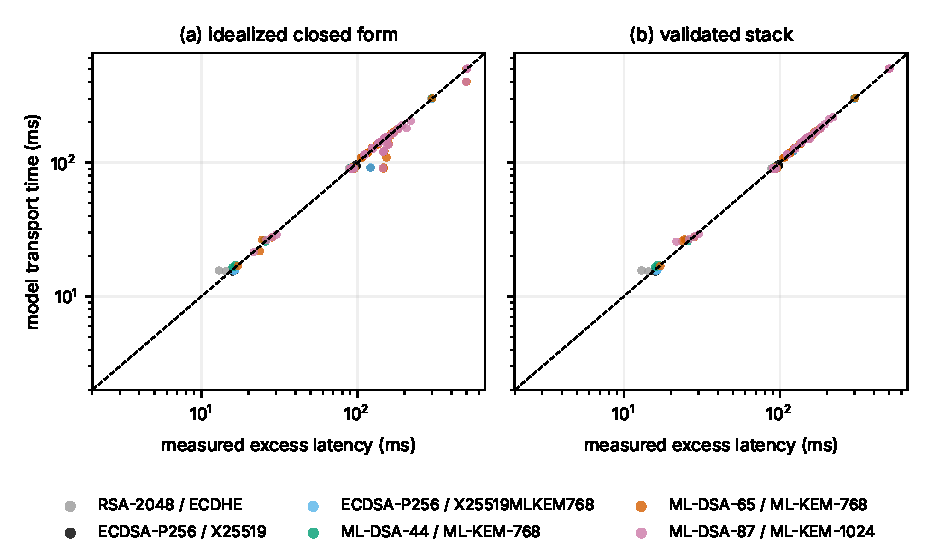
\includegraphics[width=0.8\textwidth]{figures/fig_testbed}
\caption{Measured excess latency against model prediction.}
\label{fig:testbed}
\end{figure}

\begin{table}[t]
\centering\small
\caption{Excess-latency MAE by measured suite.}
\label{tab:testbed}
\begin{tabular}{@{}>{\raggedright\arraybackslash}p{0.30\textwidth}rrrr@{}}
\toprule
\shortstack[l]{Signature /\\key exchange} & \shortstack[r]{Config-\\urations} & \shortstack[r]{MAE idealized\\(ms)} & \shortstack[r]{MAE stack\\(ms)} & \shortstack[r]{Within\\1\,ms} \\
\midrule
RSA-2048 / ECDHE & 12 & 0.95 & 0.95 & 6 of 12 \\
ECDSA-P256 / X25519 & 63 & 1.96 & 1.48 & 36 of 63 \\
ECDSA-P256 / X25519MLKEM768 & 15 & 2.59 & 0.64 & 15 of 15 \\
ML-DSA-44 / ML-KEM-768 & 12 & 0.66 & 0.72 & 9 of 12 \\
ML-DSA-65 / ML-KEM-768 & 62 & 7.02 & 1.89 & 23 of 62 \\
ML-DSA-87 / ML-KEM-1024 & 62 & 7.18 & 2.14 & 21 of 62 \\
\midrule
All & 226 & 4.70 & 1.65 & 110 of 226 \\
\bottomrule
\end{tabular}
\end{table}

\subsection{Measured TCP-proxy effect}
The term $T_\mathrm{pen}$ of \cref{eq:latency} applies only when a middlebox delays long flights. On the direct path, the least-squares fit gives $\pi=0.00$\ms at $\theta=1$ segment. Its RMSE is 2.16\ms, equal to the RMSE at $\pi=0$. The threshold-delay term does not improve the fit. We then inserted HAProxy~2.8 as a TCP proxy between the two namespaces in two modes. In the first mode, the proxy forwards bytes on arrival. In the second mode, it waits for the complete ClientHello before routing. The test covers 16 configurations: ECDSA-P256, ML-DSA-44, ML-DSA-65 and ML-DSA-87 at chain depths 1--4, a 30\ms RTT, 100\Mbits, an MTU of 1\,500\,bytes and an initial window of 10 segments, with flights of 2--27 segments. The proxy adds a mean of 0.18\ms (range $-0.22$ to 0.31\ms) in the first mode and 0.28\ms (range $-0.50$ to 0.55\ms) in the second mode. No large size-dependent delay appears in this sample. The check covers one proxy and one version. The swept values of $\pi$ up to 24\ms represent untested devices such as deep packet inspection, TLS-terminating proxies or hardware firewalls. The measurements support $\pi=0$, which the single values below use.

\section{Model-based protocol analysis}
\label{sec:results}
An operator who migrates a SWIFT~MX gateway to ML-DSA-65 must know which bytes and which round trips are added by the migration. This section reports model predictions for this question, with the model evaluated on the testbed in \cref{sec:testbed}. \Cref{tab:master} summarizes transaction size, chain-depth cost, the comparison of transport overhead with computation and compression. Its size and depth columns refer to SWIFT~MX. Its shares $\phi$ (\cref{eq:share}) use the equally weighted cold grid, separately for $\pi=0$ and for all assumed delays. These quantities refer to representative protocol profiles. They are not measured institutional transactions. \Cref{sec:sens,sec:rq5} examine their dependence on the model inputs. The results of this section are a model-based scenario analysis: \cref{tab:evidence} states which part of the study was measured and which part is model output.

\begin{table}[t]
\centering\small
\caption{Evidence level of the results.}
\label{tab:evidence}
\renewcommand{\arraystretch}{1.05}
\begin{tabularx}{\textwidth}{@{}>{\raggedright\arraybackslash}p{0.52\textwidth}>{\raggedright\arraybackslash}X@{}}
\toprule
Result & Evidence \\
\midrule
Excess latency of six suites, depth 1--4, ISO~8583-sized requests and one SWIFT-sized request (\cref{sec:testbed}) & Measured on real OpenSSL~3.5 transactions over an emulated link \\
CUBIC, delayed acknowledgments, timestamps, HAProxy (\cref{sec:testbed}) & Measured on subsets of the grid; BBR exploratory \\
Falcon, SLH-DSA and composite suites & Model, with measured certificate sizes and CPU costs; not run as TLS transactions \\
ISO~20022, SWIFT~MX, OAuth~2.0, OIDC and FAPI~2.0 profiles & Model, with measured sizes of signed objects (\cref{tab:app}); no transaction of these profiles was run \\
$\pi>0$, CPU scale above 4, windows above 32 segments, uncertainty intervals & Assumption-based \\
\bottomrule
\end{tabularx}
\end{table}

\begin{table}[t]
\centering\small
\caption{Model predictions by suite.}
\label{tab:master}
\resizebox{\textwidth}{!}{\begin{tabular}{@{}lrrrrr@{}}
\toprule
Suite & Size, KiB & Depth: $T_{d=4}-T_{d=1}$ & $O>T_\text{cpu}$, $\pi=0$ & $O>T_\text{cpu}$, all $\pi$ & Cert.\ bytes \\
 & (factor) & (ms) & (\% of rows) & (\% of rows) & compressed (\%) \\
\midrule
RSA-2048 & 27.2 (1.2$\times$) & 0.6 & 27.5 & 45 & 22 \\
RSA-3072 & 30.0 (1.3$\times$) & 0.9 & 27.3 & 44 & 18 \\
ECDSA-P256 (baseline) & 23.0 (1.0$\times$) & 29.6 & 44.2 & 51 & 31 \\
ECDSA-P256 + hybrid KEM & 25.2 (1.1$\times$) & 29.6 & 46.5 & 56 & 31 \\
ML-DSA-44 & 66.3 (2.9$\times$) & 31.4 & 70.6 & 84 & 6 \\
ML-DSA-65 & 83.4 (3.6$\times$) & 60.0 & 75.6 & 87 & 5 \\
ML-DSA-87 & 106.8 (4.6$\times$) & 32.3 & 79.4 & 93 & 3 \\
Falcon-512 & 39.9 (1.7$\times$) & 1.2 & 63.4 & 80 & 12 \\
Falcon-1024 & 56.4 (2.4$\times$) & 30.9 & 72.7 & 85 & 7 \\
SLH-DSA-128s & 126.3 (5.5$\times$) & 32.7 & 0.3 & 0 & 3 \\
SLH-DSA-128f & 246.7 (10.7$\times$) & 64.9 & 70.6 & 84 & 2 \\
ML-DSA-44+ECDSA-P256 & 67.9 (2.9$\times$) & 31.7 & 69.0 & 84 & 6 \\
ML-DSA-65+ECDSA-P256 & 84.9 (3.7$\times$) & 60.4 & 73.2 & 85 & 4 \\
\bottomrule
\end{tabular}}
\end{table}

\subsection{Authentication-byte composition}
The purpose of this analysis is to locate the bytes that post-quantum authentication adds. The configuration is a cold transaction at each protocol's reference depth. ML-DSA-65 with ML-KEM-768 enlarges a cold SWIFT~MX transaction from 23.0 to 83.4\,KiB. Falcon-512 yields 39.9\,KiB and SLH-DSA-128f yields 246.7\,KiB. \Cref{fig:sizes} shows the composition for SWIFT~MX at depth~3 and FAPI~2.0 at depth~2. For ML-DSA-65, certificate chains account for 42\% of the bytes, XMLDSig signatures and embedded certificates for 30\%, \texttt{CertificateVerify} for 8\% and the payment payload for 17\%. Lean protocols grow most. ISO~8583 grows by a factor of 6.8 with ML-DSA-65, since its handshake chains dwarf a 300-byte authorization. ISO~20022 grows 4.4 times and FAPI~2.0 grows 5.7 times (\cref{tab:sizes}). The hybrid key share adds 2.2\,KiB. On a warm connection, ISO~8583 does not grow, since it uses a symmetric MAC. ISO~20022 grows 3.1 times and FAPI~2.0 grows 4.8 times on a warm connection, since their application-layer signatures remain.

\begin{figure}[t]
\centering
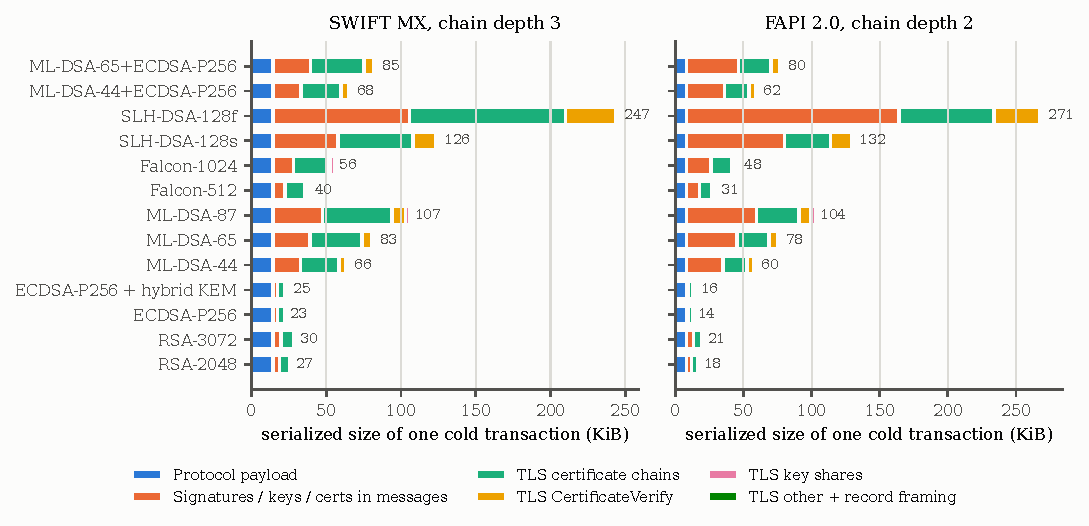
\includegraphics[width=0.8\textwidth]{figures/fig_sizes}
\caption{Composition of a cold transaction (KiB).}
\label{fig:sizes}
\end{figure}

\subsection{Chain depth and round-trip thresholds}
\Cref{fig:depth} shows SWIFT~MX latency against chain depth for three MTUs at 100\Mbits, a 30\ms RTT and $\pi=0$, on a logarithmic scale. The latency grows in whole RTTs. The classical baseline gains $+29.6$\ms from depth 1 to 4, about one RTT. From depth~2, its client flight, a handshake flight followed by a separately written request of about 11\,KiB, exceeds the initial window of ten segments. ML-DSA-65 gains $+60.0$\ms, two RTTs. Slow-start waiting contributes 56.5\ms, serialization 2.9\ms and computation 0.6\ms. The post-quantum-specific cost of three simultaneous depth increments is the difference, 30.5\ms (computed from unrounded values), or about 10.2\ms per simultaneous chain-depth increment. We define the average increment as $\bar{\Delta}_d=(T_{d=4}-T_{d=1})/3$. It averages three increments at the two peers. It is not the marginal cost of one certificate. For ML-DSA-65 at an MTU of 1\,500\,bytes, $\bar{\Delta}_d=20.0$\ms in absolute terms (3.3\ms at a 5\ms RTT and 66.7\ms at a 100\ms RTT). Jumbo frames (MTU of 9\,000\,bytes) reduce it to 1.1\ms. A delay of $\pi=24$\ms raises the jumbo-frame value to 9.1\ms (\cref{tab:depth,tab:interaction,tab:threshold}). An initial window of 32 segments halves the depth effect to $+29.9$\ms. The two chains contribute separately (\cref{tab:asym}): growing only the server chain from depth 1 to 4 adds 30.7\ms and only the client chain 29.3\ms, which sum to the 60.0\ms. Each chain pays one RTT, at different depths, since each direction has its own window.

The location of each flight depends on the stack (\cref{sec:testbed}). The idealized model produces three artifacts. It makes the hybrid suite faster than the baseline at an MTU of 1\,280\,bytes (92 vs.\ 121\ms). It gives the composite suite $+32.8$\ms against $+59.9$\ms for ML-DSA-65. It predicts a flat classical baseline ($+0.6$\ms). The stack model removes these artifacts. The hybrid suite is not faster than the baseline (122 vs.\ 121\ms); the testbed measures 121.2 vs.\ 121.0\ms on SWIFT-sized transactions. The composite suite follows ML-DSA-65 ($+60.4$ vs.\ $+60.0$\ms), and the baseline pays one RTT. ML-DSA-87 shows a smaller depth effect than ML-DSA-65 ($+32.3$ vs.\ $+60.0$\ms) in the two models, since its flights already cross an additional window boundary at depth~1. The gap between post-quantum and classical suites does not depend on these details (\cref{sec:sens}).

\begin{figure}[t]
\centering
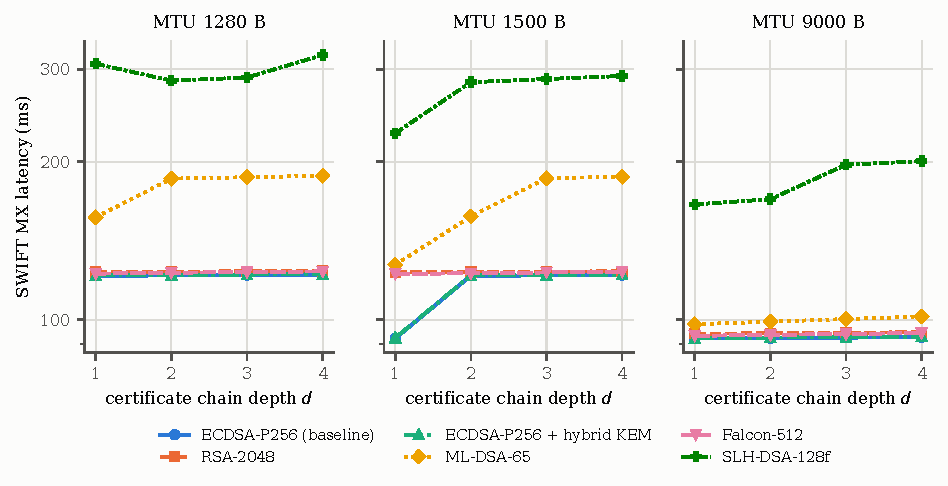
\includegraphics[width=0.75\textwidth]{figures/fig_depth}
\caption{SWIFT~MX latency against chain depth.}
\label{fig:depth}
\end{figure}

\subsection{Transport overhead and modeled cryptographic time}
The purpose of this comparison is to decide whether the size-dependent transport overhead $O$ or the modeled cryptographic primitives $T_\cpu$ dominate the added latency. $T_\cpu$ is the sum of the primitive operations on the serial critical path of the model. It excludes HSMs, middleware, queues, databases and backend processing, so a share above one half does not mean that the network takes more time than the gateway as a whole. The metric is $\phi$ of \cref{eq:share}, a fraction of equally weighted grid rows. It is not a probability or a share of the transactions of any bank. With $\pi=0$, $O>T_\cpu$ holds in 44.2\% of the baseline rows and in 75.6\% of the ML-DSA-65 rows. With all assumed delays, the shares are 51\% and 87\% (\cref{tab:master}). Nonzero delays are hypothetical sensitivity inputs; the HAProxy measurements do not support them.

With the measured x86 primitive costs, the all-delay shares are 38\% for the baseline, 66\% for Falcon-512 and 78\% for ML-DSA-65, close to the results at CPU scale 4. The serial model charges all primitive steps on its critical path; an assumed overlap that removes half or three-quarters of this charge raises the all-delay ML-DSA-65 share to 91\% and 94\%. This is an arithmetic sensitivity check, not a measurement of overlap.

\Cref{fig:ratio} shows the ratio of transport overhead to cryptographic time for the reference SWIFT~MX profile with $\pi=0$. Above 100\Mbits, the ratio changes little with the bit rate. The remaining ACK waiting depends on flight size, window state and RTT. SLH-DSA-128s is the main computation-bound exception. Its four online signatures contribute most of the 685\ms primitive budget per transaction. SLH-DSA-128f produces larger authentication traffic. The result concerns the selected implementations and protocol operations. It excludes backend payment processing.

\begin{figure}[t]
\centering
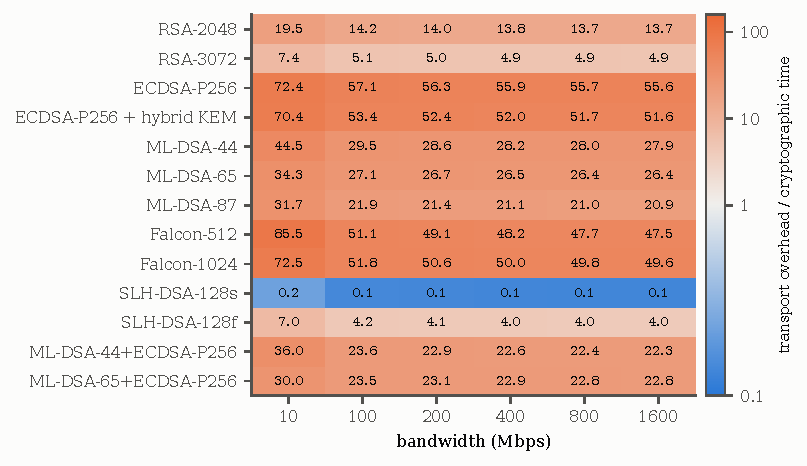
\includegraphics[width=0.6\textwidth]{figures/fig_ratio}
\caption{Transport-to-cryptographic-time ratio, SWIFT~MX.}
\label{fig:ratio}
\end{figure}

\subsection{Certificate compression and decompression cost}
Keys and signatures are pseudorandom and do not compress. Compression removes 31\% of an ECDSA-P256 chain and 5\% of an ML-DSA-65 chain. It saves at least 1\ms in only 5--21\% of the configurations. The gain depends on whether compression moves a flight below a window boundary. For ML-DSA-65, the maximum saving on this grid is about one RTT. Other suites exceed this bound (\cref{tab:rq4}). Decompression can cost more than compression saves. At an assumed client decompression rate of 3.3\,MB/s, compression is net-harmful in 95\% of the ML-DSA-65 configurations and in 0\% of the ECDSA-P256 configurations. The median break-even decompression rate for ML-DSA-65 is about 13\,MB/s (\cref{tab:rq4,fig:cc}). Zlib at level 9 reduces real ML-DSA and SLH-DSA chains to 0.88--0.98 of their size, within 0.05 of the modeled ratio (\cref{tab:comp_real}).

\subsection{Sensitivity to model inputs}
\label{sec:sens}
We varied the certificate metadata (600--1\,400\,bytes per leaf), the XMLDSig certificate embedding and the window of reused connections (\cref{tab:sens}). Omission of the signer certificate from XMLDSig reduces the ML-DSA-65 SWIFT~MX transaction from 83.4 to 67.2\,KiB. A reused connection that keeps a large window ($c=64$) reduces the warm ML-DSA-65 ISO~20022 exchange from 92 to 34\ms (baseline: 31\ms). Individual RTT steps move with these parameters. The reference comparisons keep the order Falcon-512 $<$ ML-DSA-65 $<$ SLH-DSA-128f in the evaluated input variants; this order compares selected parameter sets and is not universal over security categories or stacks.

A variance-based global sensitivity analysis over the full factorial designs computes first- and second-order indices (\cref{tab:sobol}). The RTT explains 0.59 of the variance of log latency, and the suite explains 0.28. For the post-quantum factor of the lattice schemes, the MTU explains 0.18, the RTT 0.20 and the suite 0.16.

\subsection{Assumption-based uncertainty analysis}
\label{sec:rq5}
The deterministic model propagates selected input uncertainty. Structural model error and unmeasured deployment conditions remain outside this analysis. We drew 4\,000 samples of five inputs with fixed seed 1 (\cref{tab:priors}): the certificate metadata (600--1\,400\,bytes per leaf), the CPU scale (log-uniform on $[1,16]$, an assumed range of primitive-processing slowdowns), $\pi\in[0,24]$\ms, $\theta\in[2,16]$ segments and the initial window (10, 32 or 64 segments with probabilities 0.6, 0.3 and 0.1). For each sample, we recomputed a SWIFT~MX transaction at depth~2, 100\Mbits and a 30\ms RTT (\cref{tab:uncertainty}). These priors are our assumptions. They are not fitted distributions. The resulting intervals are conditional on the priors and are not confidence intervals for the performance of any bank. They exclude structural uncertainty from other operating systems, TLS libraries and middleboxes, jitter, packet loss and institution-specific traffic.

The order Falcon-512 $<$ ML-DSA-65 $<$ SLH-DSA-128f holds in 100\% of the draws. Size-dependent transport overhead exceeds the modeled primitive time in 91\% of the draws: 99\% for CPU scales below 4 and 73\% for scales of 12--16. The ML-DSA-65 latency factor relative to the baseline has a median of 1.46 (90\% interval: 1.19--1.72). The Falcon-512 factor has a median of 1.05 (1.01--1.23). We measure input influence with the Spearman rank correlation coefficient $\rho$. For the factor, the CPU scale ($\rho=0.54$) and $\pi$ ($\rho=0.47$) dominate the initial window ($\rho=-0.36$). For $\bar{\Delta}_d$, the initial window dominates ($\rho=-0.74$). The average of about 20\ms per simultaneous ML-DSA-65 depth increment holds for the default window of 10 segments (median 22.5\ms, 90\% interval 20.1--28.4\ms). With 32 segments, the median is 12.4\ms (10.1--18.2\ms). With 64 segments, it is 3.4\ms (1.3--9.5\ms). The depth cost depends on the initial window. It is not a universal per-certificate constant. The testbed found no delay for a TCP proxy (\cref{sec:testbed}), and the intervals with nonzero $\pi$ contain hypothetical behavior of untested devices. With $\pi$ fixed at 0 and the other draws unchanged, the size-dependent overhead exceeds the modeled primitive time in 71\% of the draws (80\% for CPU scales below 4 and 59\% for 12--16), the ML-DSA-65 factor has a median of 1.33 (90\% interval 1.09--1.54), the Falcon-512 factor 1.02 (1.01--1.03), the order of the three schemes still holds in 100\% of the draws, and the median depth cost per simultaneous increment is 20.7, 10.7 and 1.8\ms at initial windows of 10, 32 and 64 segments. The 91\% above therefore depends on the hypothetical $\pi$.

\section{Discussion}
\label{sec:discussion}

\subsection{Contribution and deployment implications}
A gateway operator who plans an ML-DSA-65 migration needs the round trips that each authentication object adds. The empirical contribution of this study is the reduction of configuration-level excess-latency error, from 4.70\ms to 1.65\ms MAE, after the model accounts for write boundaries and window validation. Prior work identified authentication size and the initial window as the relevant factors; the present measurements connect them to the individual flights that incur additional ACK waiting. The MAE of 2.04\ms on the later off-grid configurations supports the abstraction over the tested bit rates, MTUs and initial windows, and the remaining systematic error limits the interpretation of predicted differences of a few milliseconds.

The application layer matters. mTLS certificate chains account for 42\% of the reference ML-DSA-65 SWIFT~MX bytes and signed application objects with embedded certificates for 30\%. A reference to the signer certificate reduces the modeled transaction from 83.4 to 67.2\,KiB, and a retained larger window reduces the modeled warm ISO~20022 exchange from 92 to 34\ms. Deployment decisions therefore start from the actual certificate path, application envelope and connection lifecycle. Operators can remove unnecessary transmitted certificates and redundant embedding where trust and protocol requirements allow. On controlled paths, a larger initial window or MTU can remove RTT steps, subject to checks of path support, congestion effects and other flows. The study establishes no universally best intervention and no maximum acceptable chain depth.

Signature selection depends on security category and implementation constraints. Falcon-512 has smaller modeled authentication traffic than ML-DSA-65, but the two do not form an equal-security comparison. SLH-DSA-128s is computation-bound under the measured primitive implementation, and SLH-DSA-128f produces substantially more traffic. These results quantify performance costs for the evaluated parameters. They do not establish deployment readiness or an exclusive role for hash-based signatures. \Cref{tab:status} records the specifications and measured components.

\subsection{Evidence boundaries and limitations}
The main empirical comparison uses one Linux/OpenSSL stack, a single x86 host with isolated network namespaces, no configured packet loss and no cross traffic. The testbed validates excess latency for request-response probes, mainly with ISO~8583-sized messages and one SWIFT-sized comparison. It does not validate ISO~20022 or FAPI workflows against operational services. The CUBIC, delayed-acknowledgment, and timestamp runs extend the tested TCP settings but do not establish transferability to other operating systems, TLS libraries, or kernel versions. BBR was checked in eight exploratory configurations and lies outside the model. The scheme order on untested stacks is not established. The link between the stack and financial deployments is an assumption of scope: gateways and API services that terminate TLS over TCP are exposed to the same two mechanisms, but we did not measure whether Linux/OpenSSL represents the Java, appliance or mainframe stacks of financial networks. On another stack the round trips may fall at other flights; the model needs only the write pattern of the library and the window rule of the kernel to be replaced.

The testbed and the model use full handshakes without session tickets, whereas production servers issue them. In a follow-up experiment, a full transaction that also issued one ticket was half a round trip slower in 6 of 40 configurations and equal in the others (\cref{tab:ticket}). The latencies reported here may therefore be up to half a round trip too low where tickets are issued, and the model has no mode for it.\par The CPU clock was fixed (\texttt{performance} governor, turbo disabled) for all campaigns reported here, so frequency changes are unlikely to explain the residual. Subtraction of unshaped medians reduces shared local processing costs. It cannot guarantee the cancellation of scheduling or network--computation overlap. Only 46 of 226 model predictions lie inside the measured 95\% bootstrap interval. The low MAE does not indicate agreement within measurement uncertainty.

The byte and CPU inputs are measured for the supported components. Falcon, SLH-DSA, and composite configurations did not run as full TLS transactions, and composite values use sums of constituent sizes and CPU costs. Protocol message sizes and the default XMLDSig certificate embedding are scenario choices. The main sweep gives both mTLS endpoints the same chain depth (\cref{tab:asym} varies them separately), and chains in which a certificate of one algorithm is signed by a CA of another algorithm are not modeled. $\bar{\Delta}_d$ measures an average simultaneous depth increment that adds a certificate at each endpoint. It does not measure the marginal delay of one certificate.

A direct measurement of an event-driven OpenSSL~3.5.4 server (\cref{tab:srvcpu}) puts the CPU per handshake at 1.18--1.35 times the primitive costs of the model for the post-quantum and RSA suites and at 1.8--2.8 times for the classical ECDSA suites, within the CPU scales of 1 to 16 swept here. No HSM, middleware, queue, database or backend payment process was measured. Project Leap Phase~2 reports receiver-side verification of 209.9\ms for its integrated Dilithium application~\cite{bis_leap2025}, much larger than the primitive costs here; its processing scope and algorithms differ. The finding that size-dependent transport overhead exceeds the modeled primitive time applies to the modeled operations. It does not apply to all processing behind a payment gateway.

HAProxy is the only measured intermediary. Its sub-millisecond added delay does not validate nonzero threshold delays for deep packet inspection, TLS termination or hardware firewalls. The sensitivity term does not model connection rejection. Packet loss, receive-window limits, wide-area jitter, competing traffic and operational tail latency remain unvalidated. Bit rates above 1\,Gbit/s and RTTs outside 5, 30 and 100\ms are model extrapolations. The 90\% uncertainty intervals are conditional on assumed input distributions. They are not confidence intervals for a population of financial deployments.

Extending the scope of the predictions requires validation on other TLS libraries and kernels, on wide-area paths with loss and cross traffic, and on operational payment gateways with HSMs.

\section{Conclusion}
\label{sec:conclusion}
Post-quantum authentication changes transport latency when certificate and application-signature bytes move a flight across the available TCP window. A model that incorporates the observed OpenSSL write pattern and Linux-style window validation locates these crossings on the tested stack. It predicts configuration-level excess latency with an MAE of 1.65\ms across 226 testbed configurations; the idealized model gives 4.70\ms. The later off-grid configurations yield an MAE of 2.04\ms, and 46 of 226 predictions fall within the measured 95\% bootstrap interval. The model retains a systematic residual of a few milliseconds.

With zero added middlebox delay, size-dependent transport overhead exceeds the modeled cryptographic-primitive time in 75.6\% of the equally weighted ML-DSA-65 cold grid. In the reference SWIFT~MX scenario, increasing the two ML-DSA-65 chain depths from 1 to 4 adds 60.0\ms, and slow-start waiting contributes 56.5\ms. The depth cost depends on the initial window and is not a constant per certificate. The mTLS chains and the application signatures each contribute to the transport cost. Connection reuse, reduced certificate embedding and suitable window settings avoid some RTT steps, whereas zlib compression helps little. These results concern the selected profiles and the modeled operations. Future work will validate the model on other TLS stacks, wide-area paths and operational payment gateways.

\section*{Data availability}
The simulator, the independent discrete-event cross-check, the measurement and testbed scripts, the raw testbed measurements (6\,960 transactions), the x86 and Arm CPU measurements, the unit tests, the scripts that regenerate the model outputs, tables and figures, the sources of this manuscript and the source of each headline number (\texttt{manuscript/data/claim\_checks.csv}) are available at \url{https://github.com/tronghieudinh/pqc-financial-transport}. The Zenodo archive \cite{dinh2026artifact} (concept DOI \href{https://doi.org/10.5281/zenodo.23839449}{10.5281/zenodo.23839449}) holds the same code and data. The test private keys of the generated certificate chains are not distributed; \texttt{certs.sh} regenerates them. Institutional traces and certificate chains of financial networks are not public and were not used.

\section*{Declarations}
\textbf{CRediT authorship contribution statement:}
\textbf{Trong-Minh Hoang:} Supervision, Resources, Formal analysis, Writing -- review \& editing.
\textbf{Trong-Hieu Dinh:} Conceptualization, Methodology, Software, Investigation, Formal analysis, Data curation, Visualization, Writing -- original draft, Writing -- review \& editing.

\textbf{Funding:} [to be completed by the authors before submission].\par\textbf{Declaration of competing interest:} The authors declare no known competing financial interests or personal relationships that could have appeared to influence the work reported in this paper.

\section*{Declaration of generative AI and AI-assisted technologies in the manuscript preparation process}
During the preparation of this work, T.-H. Dinh used Claude (Anthropic) to assist with simulation and analysis code and manuscript preparation. ChatGPT (OpenAI) and Claude (Anthropic) assisted with language revision of this manuscript and with consistency checks against the supplied data. After using these tools, the authors reviewed and edited the content as needed and take full responsibility for the content of the publication.

%% ============================================================================================
\appendix
\counterwithin*{table}{section}\counterwithin*{figure}{section}

\section{Model inputs}
\label{app:inputs}
The appendix tables combine retained measurements and regenerated model outputs. The analysis scripts produce the numerical entries. Size outputs use KiB (1\,024\,bytes). Unless stated otherwise, the configuration is 100\Mbits, a 30\ms RTT, an MTU of 1\,500\,bytes, $\pi=0$ with $\theta=4$ segments, a cold connection and the baseline ECDSA-P256 with X25519. The tables fall into three evidence classes. Measured: \cref{tab:cpu,tab:certs,tab:comp_real,tab:tls,tab:internet,tab:app,tab:cpux86,tab:residuals,tab:variants,tab:ticket,tab:srvcpu} and \cref{fig:residuals}. Model with measured inputs, validated on the testbed for the stack of \cref{sec:testbed}: \cref{tab:protocols,tab:constants,tab:sizes,tab:depth,tab:interaction,tab:threshold,tab:rq4,tab:sens,tab:rq3,tab:warm,tab:sobol} and \cref{fig:cc}. Assumption-based: \cref{tab:uncertainty} and every row that sweeps a parameter that no standard or measurement fixes (the middlebox delay, the CPU scale above the measured value and the initial window beyond the measured values). \Cref{tab:status} is a status table. The idealized model appears only in columns labeled as such.

\Cref{tab:protocols} defines the six profiles. The request and response sizes are algorithm-independent bytes summed over all exchanges, and $d_\mathrm{ref}$ is the reference chain depth. The abbreviations are BAH (Business Application Header), LAU (SWIFT Local Authentication), PAR (Pushed Authorization Request), JAR (JWT-Secured Authorization Request), JWT (JSON Web Token) and JWK(S) (JSON Web Key (Set)). \Cref{tab:constants} lists the model constants that the cited standards do not fix; all constants are overridable.

\begin{table}[!htbp]\centering\small
\caption{Financial protocol profiles.}
\label{tab:protocols}
\resizebox{\textwidth}{!}{\begin{tabularx}{\textwidth}{@{}>{\raggedright\arraybackslash}p{0.11\textwidth}>{\raggedright\arraybackslash}p{0.16\textwidth}>{\raggedright\arraybackslash}Xr>{\raggedright\arraybackslash}p{0.15\textwidth}cr@{}}
\toprule
Profile & Message types & Security objects (signer) & Exch. & Req./resp. (B)$^{a}$ & mTLS & $d_\text{ref}$ \\
\midrule
ISO 8583 & 0200/0210 & none (symmetric MAC) & 1 & 302/222 & yes & 2 \\
ISO 20022 & pacs.008 / pacs.002 & XMLDSig on BAH (client, server) & 1 & 4\,200/1\,900 & yes & 2 \\
SWIFT MX & cross-border pacs.008 & XMLDSig / LAU (client, server) & 1 & 9\,950/3\,100 & yes & 3 \\
OAuth 2.0 & RFC 6749 token + RFC 6750 call & client assertion, access token, Bearer & 2 & 1\,200/1\,320 & no & 2 \\
OIDC & token, JWKS, userinfo & client assertion, ID/access token, JWK & 3 & 1\,500/1\,220 & no & 2 \\
FAPI 2.0 & PAR, token, resource & JAR, DPoP$\times$2, tokens, signed response & 3 & 2\,000/1\,750 & yes & 2 \\
\bottomrule
\end{tabularx}}
\end{table}

\begin{table}[!htbp]\centering\small
\caption{Model constants.}
\label{tab:constants}
\resizebox{\textwidth}{!}{\begin{tabularx}{\textwidth}{@{}>{\raggedright\arraybackslash}p{0.27\textwidth}>{\raggedright\arraybackslash}X@{}}\toprule
Quantity & Value \\\midrule
Certificate metadata (leaf / CA) & 900 / 520\,bytes (sensitivity: 600/350 and 1\,400/800) \\
SPKI framing & 22\,bytes (post-quantum), 24 (RSA), 26 (ECDSA) \\
ClientHello / ServerHello without key share & 250 / 91\,bytes (calibrated on OpenSSL 3.5.4) \\
EncryptedExtensions / CertificateRequest & 10 / 53\,bytes (calibrated on OpenSSL 3.5.4) \\
Finished & 48-byte verify\_data (TLS\_AES\_256\_GCM\_SHA384) \\
TLS record framing & one record per handshake message; 22\,bytes per record of up to 16\,384\,bytes \\
IP + TCP headers & 60\,bytes (IPv6) \\
Initial / reused-connection window & 10 / 10 segments (sensitivity: 32 and 64) \\
XMLDSig fixed part & 750--800\,bytes + base64 signature + base64 signer certificate \\
Compression ratio of DER metadata & 0.68 (first certificate), 0.52 (subsequent); keys and signatures incompressible \\
Client decompression rate & 330, 33, 3.3, 0.33\,MB/s \\
Composite signature & concatenated public keys and signatures, summed CPU times \\
TCP stack behavior & Linux-style window validation (tracked peak outstanding segments; model abstraction) and the OpenSSL write pattern (4\,096-byte handshake buffer, request as a separate write, \texttt{TCP\_NODELAY}); the idealized model is the comparison baseline \\
Middlebox delay $\pi$ / threshold $\theta$ & 0--24\,ms, reference 0 / 4 segments (2--16 in a dedicated run) \\
\bottomrule\end{tabularx}}
\end{table}

\FloatBarrier
\section{Model results}
\label{app:results}
\Cref{tab:sizes} gives the serialized size of one cold transaction at the reference depth of each protocol, with the factor over the baseline in parentheses. \Cref{tab:depth} decomposes the SWIFT~MX depth increase from 1 to 4 into serialization (ser.), slow-start waiting (wait) and middlebox delay (pen.). \Cref{tab:interaction} gives $\bar{\Delta}_d$ for ML-DSA-65 against $\pi$ (a) and against the RTT (b). \Cref{tab:threshold} varies the segment threshold $\theta$ with a delay of 6\,ms per flight longer than $\theta$ segments.

\begin{table}[!htbp]\centering\small
\caption{Size of one cold transaction (KiB).}
\label{tab:sizes}
\resizebox{\textwidth}{!}{\begin{tabular}{@{}lrrrrrr@{}}
\toprule
Suite & ISO 8583 ($d{=}2$) & ISO 20022 ($d{=}2$) & SWIFT MX ($d{=}3$) & OAuth 2.0 ($d{=}2$) & OIDC ($d{=}2$) & FAPI 2.0 ($d{=}2$) \\
\midrule
RSA-2048 & 6.8 (1.4$\times$) & 18.2 (1.2$\times$) & 27.2 (1.2$\times$) & 8.8 (1.2$\times$) & 10.6 (1.3$\times$) & 18.1 (1.3$\times$) \\
RSA-3072 & 8.1 (1.6$\times$) & 20.5 (1.4$\times$) & 30.0 (1.3$\times$) & 9.9 (1.4$\times$) & 12.1 (1.4$\times$) & 21.0 (1.5$\times$) \\
ECDSA-P256 (baseline) & 4.9 (1.0$\times$) & 14.8 (1.0$\times$) & 23.0 (1.0$\times$) & 7.1 (1.0$\times$) & 8.4 (1.0$\times$) & 13.8 (1.0$\times$) \\
ECDSA-P256 + hybrid KEM & 7.1 (1.5$\times$) & 17.0 (1.1$\times$) & 25.2 (1.1$\times$) & 9.3 (1.3$\times$) & 10.6 (1.3$\times$) & 16.0 (1.2$\times$) \\
ML-DSA-44 / ML-KEM-768 & 25.7 (5.2$\times$) & 51.0 (3.4$\times$) & 66.3 (2.9$\times$) & 27.7 (3.9$\times$) & 33.7 (4.0$\times$) & 60.3 (4.4$\times$) \\
ML-DSA-65 / ML-KEM-768 & 33.4 (6.8$\times$) & 65.1 (4.4$\times$) & 83.4 (3.6$\times$) & 35.0 (5.0$\times$) & 43.0 (5.1$\times$) & 78.3 (5.7$\times$) \\
ML-DSA-87 / ML-KEM-1024 & 44.5 (9.0$\times$) & 84.7 (5.7$\times$) & 106.8 (4.6$\times$) & 46.1 (6.5$\times$) & 56.7 (6.8$\times$) & 103.7 (7.5$\times$) \\
Falcon-512 / ML-KEM-768 & 13.8 (2.8$\times$) & 28.9 (2.0$\times$) & 39.9 (1.7$\times$) & 14.9 (2.1$\times$) & 18.1 (2.2$\times$) & 31.0 (2.2$\times$) \\
Falcon-1024 / ML-KEM-1024 & 21.7 (4.4$\times$) & 42.4 (2.9$\times$) & 56.4 (2.4$\times$) & 21.7 (3.1$\times$) & 26.8 (3.2$\times$) & 47.6 (3.4$\times$) \\
SLH-DSA-128s / ML-KEM-768 & 52.6 (10.7$\times$) & 102.9 (7.0$\times$) & 126.3 (5.5$\times$) & 62.4 (8.8$\times$) & 73.8 (8.8$\times$) & 132.4 (9.6$\times$) \\
SLH-DSA-128f / ML-KEM-768 & 106.8 (21.7$\times$) & 205.3 (13.9$\times$) & 246.7 (10.7$\times$) & 125.6 (17.8$\times$) & 149.0 (17.8$\times$) & 270.8 (19.6$\times$) \\
ML-DSA-44+ECDSA-P256 & 26.4 (5.4$\times$) & 52.3 (3.5$\times$) & 67.9 (2.9$\times$) & 28.4 (4.0$\times$) & 34.6 (4.1$\times$) & 61.9 (4.5$\times$) \\
ML-DSA-65+ECDSA-P256 & 34.1 (6.9$\times$) & 66.3 (4.5$\times$) & 84.9 (3.7$\times$) & 35.7 (5.1$\times$) & 43.9 (5.2$\times$) & 80.0 (5.8$\times$) \\
\bottomrule
\end{tabular}}
\end{table}

\begin{table}[!htbp]\centering\small
\caption{SWIFT~MX latency against chain depth (ms).}
\label{tab:depth}
\resizebox{\textwidth}{!}{\begin{tabular}{@{}lrrrrrrrrr@{}}
\toprule
Suite & \multicolumn{4}{c}{Latency (ms) at depth} & \multicolumn{2}{c}{Largest flight (seg.)} & \multicolumn{3}{c}{$T_{d=4}-T_{d=1}$ components (ms)} \\
\cmidrule(lr){2-5}\cmidrule(lr){6-7}\cmidrule(lr){8-10}
 & 1 & 2 & 3 & 4 & $d{=}1$ & $d{=}4$ & ser. & wait & pen. \\
\midrule
RSA-2048 & 123.1 & 123.4 & 123.5 & 123.7 & 12 & 14 & 0.5 & 0.0 & 0 \\
RSA-3072 & 127.2 & 127.4 & 127.7 & 128.0 & 12 & 15 & 0.7 & 0.0 & 0 \\
ECDSA-P256 (baseline) & 92.1 & 121.3 & 121.5 & 121.7 & 10 & 12 & 0.3 & 29.0 & 0 \\
ECDSA-P256 + hybrid KEM & 92.4 & 121.5 & 121.7 & 121.9 & 10 & 12 & 0.4 & 29.0 & 0 \\
ML-DSA-44 & 125.2 & 126.0 & 155.8 & 156.6 & 21 & 29 & 2.1 & 28.8 & 0 \\
ML-DSA-65 & 127.3 & 157.4 & 186.1 & 187.3 & 25 & 36 & 2.9 & 56.5 & 0 \\
ML-DSA-87 & 158.3 & 187.4 & 189.0 & 190.7 & 30 & 45 & 3.9 & 27.5 & 0 \\
Falcon-512 & 122.3 & 122.6 & 123.1 & 123.5 & 14 & 19 & 1.1 & 0.1 & 0 \\
Falcon-1024 & 123.7 & 124.4 & 154.0 & 154.6 & 17 & 24 & 1.8 & 28.9 & 0 \\
SLH-DSA-128s & 868.0 & 869.5 & 871.2 & 900.7 & 36 & 53 & 4.2 & 27.5 & 0 \\
SLH-DSA-128f & 226.6 & 283.6 & 287.6 & 291.6 & 65 & 102 & 8.8 & 53.0 & 0 \\
ML-DSA-44+ECDSA-P256 & 125.6 & 126.6 & 156.4 & 157.3 & 21 & 29 & 2.2 & 28.9 & 0 \\
ML-DSA-65+ECDSA-P256 & 127.7 & 157.9 & 186.8 & 188.1 & 25 & 36 & 3.0 & 56.5 & 0 \\
\bottomrule
\end{tabular}}
\end{table}

\begin{table}[!htbp]\centering\small
\caption{ML-DSA-65 depth increment $\bar{\Delta}_d$, SWIFT~MX (ms).}
\label{tab:interaction}
\resizebox{\textwidth}{!}{\begin{tabular}{@{}lrrrrr@{\hspace{14pt}}rrrrr@{}}
\toprule
& \multicolumn{5}{c}{(a) transport penalty (ms)} & \multicolumn{5}{c}{(b) RTT (ms)} \\
\cmidrule(r){2-6}\cmidrule(l){7-11}
MTU & 0 & 3 & 6 & 12 & 24 & 5 & 12 & 30 & 50 & 100 \\
\midrule
1280 & 10.5 & 10.5 & 10.5 & 10.5 & 10.5 & 2.1 & 4.5 & 10.5 & 17.1 & 33.8 \\
1500 & 20.0 & 20.0 & 20.0 & 20.0 & 20.0 & 3.3 & 8.0 & 20.0 & 33.3 & 66.7 \\
9000 & 1.1 & 2.1 & 3.1 & 5.1 & 9.1 & 1.1 & 1.1 & 1.1 & 1.1 & 1.1 \\
\bottomrule
\end{tabular}}
\end{table}

\begin{table}[!htbp]\centering\small
\caption{Server and client chain depth varied separately: latency increase from depth 1 to 4 for SWIFT~MX (cold, mutual TLS, 100\Mbits, 30\ms RTT, $\pi=0$; ms). ``Both'' is the symmetric case of the main sweep. The server column grows only the server chain, the client column only the client chain (\texttt{asymmetric\_depth.py}).}
\label{tab:asym}
\begin{tabular}{@{}llrrrr@{}}
\toprule
Suite & Setting & Both & Server only & Client only & Sum of the two \\
\midrule
ECDSA-P256 & MTU 1\,500, window 10 & 29.6 & 0.3 & 29.3 & 29.6 \\
 & MTU 1\,500, window 32 & 0.6 & 0.3 & 0.3 & 0.6 \\
ML-DSA-65 & MTU 1\,500, window 10 & 60.0 & 30.7 & 29.3 & 60.0 \\
 & MTU 1\,500, window 32 & 29.9 & 1.8 & 28.2 & 29.9 \\
 & MTU 1\,280, window 10 & 31.4 & 1.7 & 29.7 & 31.4 \\
 & MTU 9\,000, window 10 & 3.4 & 1.7 & 1.7 & 3.4 \\
\bottomrule
\end{tabular}
\end{table}

\begin{table}[!htbp]\centering\small
\caption{Threshold sensitivity, ML-DSA-65 SWIFT~MX latency (ms).}
\label{tab:threshold}
\begin{tabular}{@{}rrrrrr@{}}
\toprule
MTU & $d$ & $\theta{=}2$ & $\theta{=}4$ & $\theta{=}8$ & $\theta{=}16$ \\
\midrule
1280 & 1 & 174.7 & 174.7 & 174.7 & 162.7 \\
 & 2 & 203.7 & 203.7 & 203.7 & 191.7 \\
 & 3 & 204.9 & 204.9 & 204.9 & 198.9 \\
 & 4 & 206.1 & 206.1 & 206.1 & 200.1 \\
\addlinespace
1500 & 1 & 145.3 & 145.3 & 139.3 & 133.3 \\
 & 2 & 175.4 & 175.4 & 175.4 & 163.4 \\
 & 3 & 204.1 & 204.1 & 204.1 & 192.1 \\
 & 4 & 205.3 & 205.3 & 205.3 & 199.3 \\
\addlinespace
9000 & 1 & 110.0 & 104.0 & 98.0 & 98.0 \\
 & 2 & 111.2 & 105.2 & 99.2 & 99.2 \\
 & 3 & 112.3 & 106.3 & 100.3 & 100.3 \\
 & 4 & 113.5 & 113.5 & 101.5 & 101.5 \\
\bottomrule
\end{tabular}
\end{table}

In \cref{tab:rq4}, a material gain is a saving of at least 1\,ms, and a net-harmful configuration has a net effect of at most $-1$\,ms at the given client decompression rate. The break-even column is the median decompression cost (ms/KiB) over configurations with a material gain. \Cref{fig:cc} plots the share of configurations with a gain (a) and with a net-harmful effect (b). \Cref{tab:sens} reports the depth effect $T_{d=4}-T_{d=1}$ for SWIFT~MX and the warm ISO~20022 latency under the input variants of \cref{sec:sens}; SLH-f denotes SLH-DSA-128f. \Cref{tab:rq3} gives the transport-bound share by CPU scale, and \cref{tab:warm} gives the added latency over the baseline on a reused connection.

\begin{table}[!htbp]\centering\small
\caption{Certificate compression.}
\label{tab:rq4}
\resizebox{\textwidth}{!}{\begin{tabular}{@{}lrrrrrrrr@{}}
\toprule
Suite & Cert.\ bytes & Material & Max saved & \multicolumn{4}{c}{Net-harmful configurations (\%) by client decompression rate} & Break-even \\
\cmidrule(lr){5-8}
 & saved (\%) & gain (\%) & (RTTs) & 330 MB/s & 33 MB/s & 3.3 MB/s & 0.33 MB/s & (ms/KiB) \\
\midrule
RSA-2048 & 22 & 16 & 9.89 & 0 & 0 & 31 & 94 & 1.70 \\
RSA-3072 & 18 & 13 & 5.79 & 0 & 0 & 35 & 97 & 1.01 \\
ECDSA-P256 (baseline) & 31 & 10 & 5.16 & 0 & 0 & 0 & 97 & 0.98 \\
ECDSA-P256 + hybrid KEM & 31 & 15 & 9.97 & 0 & 0 & 0 & 94 & 1.96 \\
ML-DSA-44 & 6 & 10 & 5.07 & 0 & 0 & 94 & 99 & 0.11 \\
ML-DSA-65 & 5 & 11 & 1.00 & 0 & 0 & 95 & 98 & 0.08 \\
ML-DSA-87 & 3 & 11 & 1.00 & 0 & 2 & 96 & 99 & 0.12 \\
Falcon-512 & 12 & 5 & 0.35 & 0 & 0 & 66 & 100 & 0.20 \\
Falcon-1024 & 7 & 21 & 1.00 & 0 & 0 & 80 & 92 & 1.60 \\
SLH-DSA-128s & 3 & 13 & 1.00 & 0 & 8 & 94 & 99 & 0.24 \\
SLH-DSA-128f & 2 & 5 & 0.36 & 0 & 64 & 100 & 100 & 0.02 \\
ML-DSA-44+ECDSA-P256 & 6 & 8 & 5.07 & 0 & 0 & 95 & 100 & 0.10 \\
ML-DSA-65+ECDSA-P256 & 4 & 6 & 0.36 & 0 & 0 & 99 & 100 & 0.07 \\
\bottomrule
\end{tabular}}
\end{table}

\begin{table}[!htbp]\centering\small
\caption{Sensitivity to model inputs (ms).}
\label{tab:sens}
\resizebox{\textwidth}{!}{\begin{tabular}{@{}lrrrrrrrr@{}}
\toprule
Variant & \multicolumn{4}{c}{$T_{d=4}-T_{d=1}$ for SWIFT MX (ms)} & \multicolumn{4}{c}{Warm ISO 20022 latency (ms)} \\
\cmidrule(lr){2-5}\cmidrule(lr){6-9}
 & ECDSA & ML-DSA-65 & Falcon-512 & SLH-f & ECDSA & ML-DSA-65 & Falcon-512 & SLH-f \\
\midrule
Reference model & 29.6 & 60.0 & 1.2 & 64.9 & 31.0 & 92.0 & 31.6 & 169.2 \\
XMLDSig without embedded certificate & 29.6 & 32.3 & 1.2 & 64.9 & 30.8 & 32.8 & 31.0 & 109.7 \\
Smaller certificates (leaf 600 B, CA 350 B) & 29.5 & 60.1 & 1.1 & 64.8 & 30.9 & 91.9 & 31.5 & 169.1 \\
Larger certificates (leaf 1400 B, CA 800 B) & 0.7 & 60.2 & 1.4 & 65.1 & 31.1 & 92.1 & 31.7 & 169.3 \\
Busy reused connection ($c=64$) & 29.6 & 60.0 & 1.2 & 64.9 & 31.0 & 34.1 & 31.6 & 55.9 \\
\bottomrule
\end{tabular}}
\end{table}

\begin{table}[!htbp]\centering\small
\caption{Transport overhead against cryptographic time.}
\label{tab:rq3}
\resizebox{\textwidth}{!}{\begin{tabular}{@{}lrrrrr@{}}
\toprule
Suite & \multicolumn{3}{c}{$O>T_\mathrm{cpu}$ (\% of rows)} & Median $O/T_\mathrm{cpu}$ & Added $O>$ added $T_\mathrm{cpu}$ \\
\cmidrule(lr){2-4}
 & CPU $\times1$ & $\times4$ & $\times16$ & ($\times1$) & vs.\ baseline, $\times1$ (\%) \\
\midrule
RSA-2048 & 45 & 35 & 12 & 0.5 & 34 \\
RSA-3072 & 44 & 19 & 4 & 0.3 & 27 \\
ECDSA-P256 (baseline) & 51 & 36 & 27 & 1.2 & -- \\
ECDSA-P256 + hybrid KEM & 56 & 39 & 30 & 1.6 & 69 \\
ML-DSA-44 & 84 & 74 & 52 & 17.3 & 84 \\
ML-DSA-65 & 87 & 76 & 50 & 16.1 & 86 \\
ML-DSA-87 & 93 & 80 & 51 & 16.7 & 94 \\
Falcon-512 & 80 & 65 & 52 & 19.2 & 89 \\
Falcon-1024 & 85 & 75 & 61 & 24.5 & 85 \\
SLH-DSA-128s & 0 & 0 & 0 & 0.1 & 0 \\
SLH-DSA-128f & 84 & 46 & 3 & 3.6 & 84 \\
ML-DSA-44+ECDSA-P256 & 84 & 73 & 48 & 14.6 & 83 \\
ML-DSA-65+ECDSA-P256 & 85 & 74 & 46 & 14.1 & 85 \\
\bottomrule
\end{tabular}}
\end{table}

\begin{table}[!htbp]\centering\small
\caption{Added latency on a reused connection (ms).}
\label{tab:warm}
\resizebox{\textwidth}{!}{\begin{tabular}{@{}lrrrrrr@{}}
\toprule
Suite & ISO 8583 & ISO 20022 & SWIFT MX & OAuth 2.0 & OIDC & FAPI 2.0 \\
\midrule
RSA-2048 & 0.0 & 1.0 & 1.0 & 0.9 & 1.4 & 2.9 \\
RSA-3072 & 0.0 & 3.1 & 3.1 & 2.9 & 4.4 & 8.9 \\
ECDSA-P256 + hybrid KEM & 0.0 & 0.0 & 0.0 & 0.0 & 0.0 & 0.0 \\
ML-DSA-44 & 0.0 & 31.0 & 31.0 & 1.6 & 2.3 & 4.4 \\
ML-DSA-65 & 0.0 & 61.0 & 61.0 & 2.4 & 3.6 & 6.9 \\
ML-DSA-87 & 0.0 & 62.0 & 62.0 & 3.2 & 4.7 & 9.0 \\
Falcon-512 & 0.0 & 0.6 & 29.5 & 0.3 & 0.5 & 1.1 \\
Falcon-1024 & 0.0 & 1.3 & 30.2 & 0.8 & 1.3 & 2.6 \\
SLH-DSA-128s & 0.0 & 403.1 & 403.1 & 344.5 & 545.2 & 1060.5 \\
SLH-DSA-128f & 0.0 & 138.2 & 138.2 & 81.3 & 119.5 & 151.2 \\
ML-DSA-44+ECDSA-P256 & 0.0 & 31.1 & 31.1 & 1.7 & 2.6 & 4.9 \\
ML-DSA-65+ECDSA-P256 & 0.0 & 61.1 & 61.1 & 2.6 & 3.9 & 7.4 \\
\bottomrule
\end{tabular}}
\end{table}

\begin{figure}[!htbp]\centering
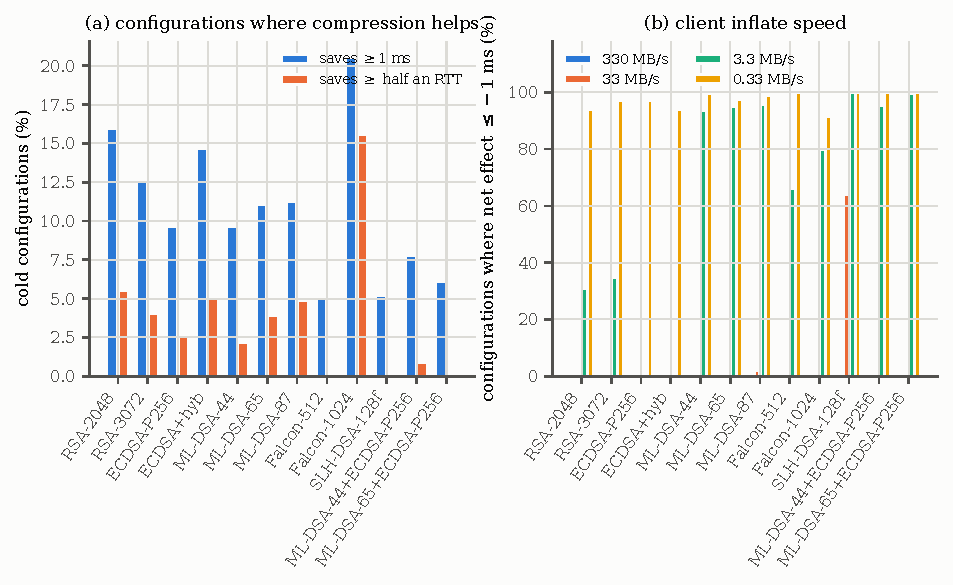
\includegraphics[width=\textwidth]{figures/fig_cc}
\caption{Effect of certificate compression.}
\label{fig:cc}
\end{figure}

\FloatBarrier
\section{Measured inputs and input checks}
\label{app:meas}
\Cref{tab:cpu} gives the per-operation medians on a performance core (Cortex-X925) and an efficiency core (Cortex-A725). \Cref{tab:certs} compares the DER sizes of the generated certificates with the sizes predicted from the ECDSA-calibrated metadata. \Cref{tab:comp_real} compares the zlib level-9 compression ratio of real chains with the model. Since the generated chains repeat names and extensions more often than public chains, classical chains compress better here than in the calibration set. \Cref{tab:tls} compares real TLS~1.3 handshake flights (OpenSSL~3.5.4, mTLS) with the calibrated model for the same certificates, and the loopback handshake time with the modeled handshake CPU time; CH denotes the ClientHello.

\begin{table}[!htbp]\centering\footnotesize
\caption{Per-operation CPU cost (ms).}
\label{tab:cpu}
\resizebox{0.92\textwidth}{!}{\begin{tabular}{@{}llrrrl@{}}
\toprule
Algorithm & Op. & X925 & A725 & A725/X925 & Implementation \\
\midrule
RSA-2048 & sign & 0.491 & 1.085 & 2.21 & OpenSSL 3.5.4 \\
RSA-2048 & verify & 0.0147 & 0.03163 & 2.15 & OpenSSL 3.5.4 \\
RSA-3072 & sign & 1.451 & 3.271 & 2.26 & OpenSSL 3.5.4 \\
RSA-3072 & verify & 0.0293 & 0.0648 & 2.21 & OpenSSL 3.5.4 \\
ECDSA-P256 & sign & 0.01446 & 0.02616 & 1.81 & OpenSSL 3.5.4 \\
ECDSA-P256 & verify & 0.04112 & 0.07835 & 1.91 & OpenSSL 3.5.4 \\
ML-DSA-44 & sign & 0.3594 & 0.753 & 2.10 & OpenSSL 3.5.4 \\
ML-DSA-44 & verify & 0.06804 & 0.1489 & 2.19 & OpenSSL 3.5.4 \\
ML-DSA-65 & sign & 0.586 & 1.225 & 2.09 & OpenSSL 3.5.4 \\
ML-DSA-65 & verify & 0.103 & 0.2289 & 2.22 & OpenSSL 3.5.4 \\
ML-DSA-87 & sign & 0.6691 & 1.438 & 2.15 & OpenSSL 3.5.4 \\
ML-DSA-87 & verify & 0.1589 & 0.3594 & 2.26 & OpenSSL 3.5.4 \\
Falcon-512 & sign & 0.1045 & 0.2057 & 1.97 & liboqs 0.14.0 \\
Falcon-512 & verify & 0.01755 & 0.0311 & 1.77 & liboqs 0.14.0 \\
Falcon-1024 & sign & 0.2114 & 0.4026 & 1.90 & liboqs 0.14.0 \\
Falcon-1024 & verify & 0.03098 & 0.05949 & 1.92 & liboqs 0.14.0 \\
SLH-DSA-128s & sign & 170.8 & 259.6 & 1.52 & OpenSSL 3.5.4 \\
SLH-DSA-128s & verify & 0.1614 & 0.2604 & 1.61 & OpenSSL 3.5.4 \\
SLH-DSA-128f & sign & 8.2 & 13.08 & 1.60 & OpenSSL 3.5.4 \\
SLH-DSA-128f & verify & 0.5058 & 0.7719 & 1.53 & OpenSSL 3.5.4 \\
\midrule
ECDHE-P256 & gen & 0.00845 & 0.01721 & 2.04 & OpenSSL 3.5.4 \\
ECDHE-P256 & derive & 0.03406 & 0.06565 & 1.93 & OpenSSL 3.5.4 \\
ECDHE-P256 & server & 0.04251 & 0.08286 & 1.95 & OpenSSL 3.5.4 \\
X25519 & gen & 0.01326 & 0.03127 & 2.36 & OpenSSL 3.5.4 \\
X25519 & derive & 0.0227 & 0.04522 & 1.99 & OpenSSL 3.5.4 \\
X25519 & server & 0.03596 & 0.07649 & 2.13 & OpenSSL 3.5.4 \\
X25519MLKEM768 & gen & 0.0311 & 0.07323 & 2.35 & OpenSSL 3.5.4 \\
X25519MLKEM768 & derive & 0.03734 & 0.08021 & 2.15 & OpenSSL 3.5.4 \\
X25519MLKEM768 & server & 0.04516 & 0.09852 & 2.18 & OpenSSL 3.5.4 \\
ML-KEM-768 & gen & 0.01784 & 0.04196 & 2.35 & OpenSSL 3.5.4 \\
ML-KEM-768 & derive & 0.01464 & 0.03499 & 2.39 & OpenSSL 3.5.4 \\
ML-KEM-768 & server & 0.0092 & 0.02203 & 2.40 & OpenSSL 3.5.4 \\
ML-KEM-1024 & gen & 0.02664 & 0.06338 & 2.38 & OpenSSL 3.5.4 \\
ML-KEM-1024 & derive & 0.01898 & 0.0458 & 2.41 & OpenSSL 3.5.4 \\
ML-KEM-1024 & server & 0.01183 & 0.02885 & 2.44 & OpenSSL 3.5.4 \\
\bottomrule
\end{tabular}}
\end{table}

\begin{table}[!htbp]\centering\small
\caption{Generated certificate sizes (bytes).}
\label{tab:certs}
\resizebox{\textwidth}{!}{\begin{tabular}{@{}lrrrrrr@{}}
\toprule
Algorithm & Leaf DER & CA DER & Metadata (leaf/CA) & Predicted leaf & Predicted CA & Max error (\%) \\
\midrule
RSA-2048 & 1416 & 1227 & 862/673 & 1408 & 1217 & 0.81 \\
RSA-3072 & 1672 & 1483 & 862/673 & 1664 & 1473 & 0.67 \\
ECDSA-P256 & 1021 & 830 & 854/663 & 1021 & 830 & 0.00 \\
ML-DSA-44 & 4616 & 4427 & 858/669 & 4612 & 4421 & 0.14 \\
ML-DSA-65 & 6145 & 5956 & 858/669 & 6141 & 5950 & 0.10 \\
ML-DSA-87 & 8103 & 7914 & 858/669 & 8099 & 7908 & 0.08 \\
SLH-DSA-128s & 8768 & 8579 & 854/665 & 8768 & 8577 & 0.02 \\
SLH-DSA-128f & 18000 & 17811 & 854/665 & 18000 & 17809 & 0.01 \\
\bottomrule
\end{tabular}}
\end{table}

\begin{table}[!htbp]\centering\small
\caption{Compression ratio of real chains.}
\label{tab:comp_real}
\resizebox{\textwidth}{!}{\begin{tabular}{@{}lrrrrrrrr@{}}
\toprule
Algorithm & \multicolumn{2}{c}{$d=1$} & \multicolumn{2}{c}{$d=2$} & \multicolumn{2}{c}{$d=3$} & \multicolumn{2}{c}{$d=4$} \\
\cmidrule(lr){2-3} \cmidrule(lr){4-5} \cmidrule(lr){6-7} \cmidrule(lr){8-9}
 & zlib-9 & model & zlib-9 & model & zlib-9 & model & zlib-9 & model \\
\midrule
RSA-2048 & 0.76 & 0.81 & 0.67 & 0.77 & 0.61 & 0.75 & 0.58 & 0.75 \\
RSA-3072 & 0.80 & 0.83 & 0.73 & 0.81 & 0.68 & 0.80 & 0.65 & 0.79 \\
ECDSA-P256 & 0.64 & 0.73 & 0.53 & 0.67 & 0.44 & 0.65 & 0.40 & 0.64 \\
ML-DSA-44 & 0.93 & 0.94 & 0.91 & 0.93 & 0.89 & 0.93 & 0.88 & 0.93 \\
ML-DSA-65 & 0.95 & 0.95 & 0.93 & 0.95 & 0.92 & 0.95 & 0.92 & 0.95 \\
ML-DSA-87 & 0.96 & 0.97 & 0.95 & 0.96 & 0.94 & 0.96 & 0.94 & 0.96 \\
SLH-DSA-128s & 0.96 & 0.97 & 0.95 & 0.96 & 0.95 & 0.96 & 0.94 & 0.96 \\
SLH-DSA-128f & 0.98 & 0.98 & 0.98 & 0.98 & 0.98 & 0.98 & 0.97 & 0.98 \\
\bottomrule
\end{tabular}}
\end{table}

\begin{table}[!htbp]\centering\small
\caption{Real TLS~1.3 handshake flights (bytes).}
\label{tab:tls}
\resizebox{\textwidth}{!}{\begin{tabular}{@{}lrrrrrrrr@{}}
\toprule
Suite (mutual TLS) & $d$ & CH & Server flight & Client flight & Model total & Error (\%) & Loopback (ms) & Model CPU (ms) \\
\midrule
RSA-2048 & 1 & 323 & 2075 & 1812 & 4202 & $-$0.19 & 2.00 & 1.13 \\
RSA-2048 & 4 & 323 & 5771 & 5508 & 11594 & $-$0.07 & 2.07 & 1.21 \\
RSA-3072 & 1 & 323 & 2459 & 2196 & 4970 & $-$0.16 & 4.21 & 3.10 \\
RSA-3072 & 4 & 323 & 6923 & 6660 & 13898 & $-$0.06 & 4.38 & 3.28 \\
ECDSA-P256 (baseline) & 1 & 290 & 1460 & 1231 & 2974 & $-$0.23 & 0.74 & 0.27 \\
ECDSA-P256 (baseline) & 4 & 290 & 3969 & 3737 & 7992 & $-$0.05 & 0.85 & 0.51 \\
ECDSA-P256 + hybrid KEM & 1 & 1466 & 2548 & 1231 & 5246 & 0.02 & 0.59 & 0.31 \\
ECDSA-P256 + hybrid KEM & 4 & 1466 & 5057 & 3737 & 10264 & 0.04 & 0.82 & 0.55 \\
ML-DSA-44 & 1 & 1434 & 8462 & 7176 & 17072 & 0.00 & 0.97 & 1.03 \\
ML-DSA-44 & 4 & 1434 & 21780 & 20494 & 43708 & 0.00 & 1.51 & 1.44 \\
ML-DSA-65 & 1 & 1434 & 10880 & 9594 & 21908 & 0.00 & 1.89 & 1.63 \\
ML-DSA-65 & 4 & 1434 & 28785 & 27499 & 57718 & 0.00 & 2.23 & 2.24 \\
ML-DSA-87 & 1 & 1818 & 14636 & 12870 & 29324 & 0.00 & 2.31 & 2.03 \\
ML-DSA-87 & 4 & 1818 & 38415 & 36649 & 76882 & 0.00 & 2.36 & 2.98 \\
\bottomrule
\end{tabular}}
\end{table}

\FloatBarrier
\section{Internet check, application objects, sensitivity, residuals and status}
\label{app:more}
\Cref{tab:internet} reports real-Internet handshakes with X25519 and X25519\allowbreak{}MLKEM768 over 100 interleaved rounds per server: median times, the paired difference with its bootstrap 95\% confidence interval and the extra bytes. \Cref{tab:app} compares real signed application objects with the model: the JWS client assertion and access token, the DPoP proof and the XMLDSig over a pacs.008 document with the signer certificate in \texttt{KeyInfo}. \Cref{tab:sobol} lists the largest first- and second-order variance-based indices of log latency and of the log post-quantum (PQ) factor over the full factorial wired designs. \Cref{tab:uncertainty} summarizes the 4\,000 draws of \cref{sec:rq5} by median and 5th and 95th percentiles; probabilities appear in the median column.

\begin{table}[!htbp]\centering\small
\caption{Real-Internet handshakes.}
\label{tab:internet}
\resizebox{\textwidth}{!}{\begin{tabular}{@{}lrrrrr@{}}
\toprule
Server & RTT (ms) & X25519 (ms) & X25519MLKEM768 (ms) & Paired difference (ms) & Extra bytes out/in \\
\midrule
cloudflare.com & 30 & 35.4 & 37.0 & 2.9 [1.2, 4.4] & 1176/1088 \\
www.google.com & 34 & 62.9 & 65.9 & 2.5 [0.1, 5.7] & 1176/1088 \\
\bottomrule
\end{tabular}}
\end{table}

\begin{table}[!htbp]\centering\small
\caption{Real signed application objects (bytes).}
\label{tab:app}
\resizebox{\textwidth}{!}{\begin{tabular}{@{}lrrrrrrrr@{}}
\toprule
Algorithm & \multicolumn{2}{c}{Client assertion} & \multicolumn{2}{c}{Access token} & \multicolumn{2}{c}{DPoP proof} & \multicolumn{2}{c}{XMLDSig} \\
\cmidrule(lr){2-3}\cmidrule(lr){4-5}\cmidrule(lr){6-7}\cmidrule(l){8-9}
 & real & model & real & model & real & model & real & model \\
\midrule
ECDSA-P256 & 381 & 536 & 549 & 796 & 518 & 732 & 2268 & 2270 \\
RSA-2048 & 637 & 782 & 805 & 1042 & 1104 & 1342 & 3055 & 3034 \\
ML-DSA-44 & 3527 & 3667 & 3695 & 3927 & 5883 & 6081 & 10182 & 10190 \\
ML-DSA-65 & 4712 & 4852 & 4880 & 5112 & 8206 & 8403 & 13406 & 13414 \\
ML-DSA-87 & 6470 & 6610 & 6638 & 6870 & 11101 & 11298 & 17774 & 17782 \\
SLH-DSA-128s & 10786 & 10915 & 10954 & 11175 & 10877 & 11053 & 22969 & 22978 \\
SLH-DSA-128f & 23095 & 23224 & 23263 & 23484 & 23186 & 23362 & 47585 & 47598 \\
\bottomrule
\end{tabular}}
\end{table}

\begin{table}[!htbp]\centering\small
\caption{Global sensitivity indices.}
\label{tab:sobol}
\resizebox{\textwidth}{!}{\begin{tabular}{@{}lp{0.68\textwidth}@{}}
\toprule
Response & Largest first- and second-order indices \\
\midrule
log latency, wired & RTT (0.59), suite (0.28), suite $\times$ RTT (0.04), protocol (0.03), MTU (0.02) \\
log PQ factor, wired, all PQ suites & suite (0.68), RTT (0.12), suite $\times$ RTT (0.09), MTU (0.02), protocol (0.01) \\
log PQ factor, wired, ML-DSA and Falcon & RTT (0.20), MTU (0.18), suite (0.16), penalty (0.09), protocol (0.06) \\
\bottomrule
\end{tabular}}
\end{table}

\begin{table}[!htbp]\centering\small
\caption{Assumption-based uncertainty, SWIFT~MX.}
\label{tab:uncertainty}
\begin{tabular}{@{}lrrr@{}}\toprule
Metric & Median & 5th pct. & 95th pct. \\\midrule
ML-DSA-65 latency (ms) & 179.6 & 115.1 & 238.5 \\
ML-DSA-65 factor over baseline & 1.46 & 1.19 & 1.72 \\
Falcon-512 factor & 1.05 & 1.01 & 1.23 \\
SLH-DSA-128f factor & 3.34 & 2.31 & 6.21 \\
SLH-DSA-128s factor & 25.6 & 8.2 & 79.4 \\
ML-DSA-65 $\bar{\Delta}_d$ (ms) & 20.5 & 3.5 & 27.9 \\
$\Pr(O>T_\mathrm{cpu})$ & 0.91 & \multicolumn{2}{c}{--} \\
$\Pr$(Falcon-512 $<$ ML-DSA-65 $<$ SLH-DSA-128f) & 1.00 & \multicolumn{2}{c}{--} \\
\bottomrule\end{tabular}
\end{table}

\Cref{tab:ablation} gives the contribution of each stack mechanism on the 226 validation configurations, and \cref{tab:priors} lists the prior distributions of the uncertainty analysis of \cref{sec:rq5} (script \texttt{uncertainty.py}, seed 1; \texttt{--pi0} fixes $\pi=0$).

\begin{table}[!htbp]\centering\small
\caption{Contribution of each stack mechanism: excess-latency prediction error on the 226 validation configurations (model minus measurement). Nothing is fitted (\texttt{ablation\_stack.py}).}
\label{tab:ablation}
\begin{tabular}{@{}lrrrr@{}}
\toprule
Model & MAE (ms) & Bias (ms) & Maximum error (ms) & Configurations above 0.4\,RTT \\
\midrule
Idealized (no mechanism) & 4.70 & $-3.5$ & 97.1 & 21 \\
Window validation only & 3.34 & $-2.0$ & 95.4 & 12 \\
OpenSSL write boundaries only & 3.15 & $-1.8$ & 95.3 & 15 \\
Both (model of this paper) & 1.65 & $+0.1$ & 5.4 & 4 \\
\bottomrule
\end{tabular}
\end{table}

\begin{table}[!htbp]\centering\small
\caption{Prior distributions of the uncertainty analysis (4\,000 draws, seed 1). The inputs are drawn independently, except that the metadata of leaf and CA certificates share one quantile and so move together. The priors are assumptions, not fitted distributions.}
\label{tab:priors}
\begin{tabular}{@{}lll@{}}
\toprule
Input & Distribution & Basis \\
\midrule
Leaf certificate metadata & uniform, 600--1\,400\,bytes & range around the calibrated 900\,bytes \\
CA certificate metadata & uniform, 350--800\,bytes (same quantile as the leaf) & range around the calibrated 520\,bytes \\
CPU scale & log-uniform, 1--16 & 1 measured X925, 4 measured x86, 16 assumed \\
Middlebox delay $\pi$ & uniform, 0--24\,ms & assumption; the HAProxy measurements support 0 \\
Segment threshold $\theta$ & uniform on the integers 2--16 & assumption \\
Initial window & 10, 32, 64 segments with probabilities 0.6, 0.3, 0.1 & RFC~6928 default and larger production windows \\
\bottomrule
\end{tabular}
\end{table}

\Cref{tab:cpux86} compares the primitive costs on the critical path for the Cortex-X925 (simulator default), the Cortex-A725 and one core of the Intel Core i7-5600U (2.5\,GHz, AVX2, turbo disabled), with the same method. \Cref{tab:residuals} and \cref{fig:residuals} break down the stack-model error (model minus measurement) by configuration group. The 95\% interval of the MAE uses 2\,000 bootstrap resamples of the configurations. The core grid is the identification set (100\Mbits, initial window of 10 segments). The off-grid set comes from a later campaign on the same day (UTC 07:51--08:35 for the core grid and 09:07--09:17 off-grid); no model parameter was fitted to it. All rows use Reno, no loss, mTLS and the direct path.

\begin{table}[!htbp]\centering\small
\caption{Primitive cost on three cores (ms).}
\label{tab:cpux86}
\begin{tabular}{@{}llrrrr@{}}
\toprule
Primitive & Operation & X925 (ms) & A725 (ms) & x86 (ms) & x86/X925 \\
\midrule
RSA-2048 & sign & 0.491 & 1.09 & 0.835 & 1.7 \\
RSA-2048 & verify & 0.0147 & 0.0316 & 0.0334 & 2.3 \\
ECDSA-P256 & sign & 0.0145 & 0.0262 & 0.0402 & 2.8 \\
ECDSA-P256 & verify & 0.0411 & 0.0783 & 0.102 & 2.5 \\
ML-DSA-44 & sign & 0.359 & 0.753 & 1.05 & 2.9 \\
ML-DSA-44 & verify & 0.068 & 0.149 & 0.213 & 3.1 \\
ML-DSA-65 & sign & 0.586 & 1.22 & 1.72 & 2.9 \\
ML-DSA-65 & verify & 0.103 & 0.229 & 0.326 & 3.2 \\
ML-DSA-87 & sign & 0.669 & 1.44 & 1.95 & 2.9 \\
ML-DSA-87 & verify & 0.159 & 0.359 & 0.508 & 3.2 \\
Falcon-512 & sign & 0.105 & 0.206 & 0.361 & 3.4 \\
Falcon-512 & verify & 0.0176 & 0.0311 & 0.065 & 3.7 \\
SLH-DSA-128s & sign & 171 & 260 & 1\,320 & 7.7 \\
SLH-DSA-128s & verify & 0.161 & 0.26 & 1.3 & 8.1 \\
SLH-DSA-128f & sign & 8.2 & 13.1 & 63.1 & 7.7 \\
SLH-DSA-128f & verify & 0.506 & 0.772 & 3.79 & 7.5 \\
X25519 & key generation & 0.0133 & 0.0313 & 0.0513 & 3.9 \\
X25519 & derive & 0.0227 & 0.0452 & 0.0509 & 2.2 \\
ML-KEM-768 & key generation & 0.0178 & 0.042 & 0.0641 & 3.6 \\
ML-KEM-768 & encapsulate & 0.0092 & 0.022 & 0.04 & 4.3 \\
ML-KEM-768 & decapsulate & 0.0146 & 0.035 & 0.0608 & 4.2 \\
\bottomrule
\end{tabular}
\end{table}

\begin{table}[!htbp]\centering\small
\caption{Stack-model error by configuration group.}
\label{tab:residuals}
\resizebox{\textwidth}{!}{\begin{tabular}{@{}llrrrrr@{}}
\toprule
Group & Value & $n$ & MAE (ms) & RMSE (ms) & MAE / mean excess (\%) & MAE 95\% interval (ms) \\
\midrule
 & all configurations & 226 & 1.65 & 2.16 & 1.2 & 1.48--1.83 \\
\midrule
 & core grid (100\,Mbit/s, initial window 10) & 82 & 0.96 & 1.34 & 0.6 & 0.77--1.18 \\
 & off-grid (later campaign) & 144 & 2.04 & 2.51 & 1.8 & 1.81--2.28 \\
\midrule
RTT (ms) & 5 & 24 & 0.95 & 1.31 & 4.9 & 0.63--1.33 \\
RTT (ms) & 30 & 178 & 1.84 & 2.34 & 1.6 & 1.63--2.05 \\
RTT (ms) & 100 & 24 & 0.92 & 1.30 & 0.2 & 0.57--1.31 \\
\midrule
MTU (bytes) & 1280 & 58 & 1.87 & 2.39 & 1.5 & 1.50--2.26 \\
MTU (bytes) & 1500 & 120 & 1.33 & 1.83 & 0.9 & 1.12--1.57 \\
MTU (bytes) & 9000 & 48 & 2.17 & 2.61 & 2.1 & 1.77--2.58 \\
\midrule
initial window & 10 & 154 & 1.32 & 1.80 & 0.9 & 1.13--1.52 \\
initial window & 32 & 72 & 2.35 & 2.79 & 2.2 & 2.01--2.70 \\
\midrule
chain depth & 1 & 60 & 1.72 & 2.21 & 1.4 & 1.36--2.06 \\
chain depth & 2 & 58 & 1.58 & 2.00 & 1.2 & 1.28--1.89 \\
chain depth & 3 & 54 & 1.59 & 2.17 & 1.1 & 1.21--1.98 \\
chain depth & 4 & 54 & 1.70 & 2.27 & 1.2 & 1.33--2.13 \\
\midrule
suite & ECDSA-P256 & 63 & 1.48 & 1.89 & 1.4 & 1.19--1.77 \\
suite & ECDSA + hybrid KEM & 15 & 0.64 & 0.64 & 0.5 & 0.60--0.67 \\
suite & ML-DSA-44 & 12 & 0.72 & 0.90 & 0.4 & 0.43--1.03 \\
suite & ML-DSA-65 & 62 & 1.89 & 2.38 & 1.4 & 1.54--2.25 \\
suite & ML-DSA-87 & 62 & 2.14 & 2.67 & 1.4 & 1.75--2.54 \\
suite & RSA-2048 & 12 & 0.95 & 1.38 & 0.7 & 0.40--1.51 \\
\bottomrule
\end{tabular}}
\end{table}

\begin{figure}[!htbp]\centering
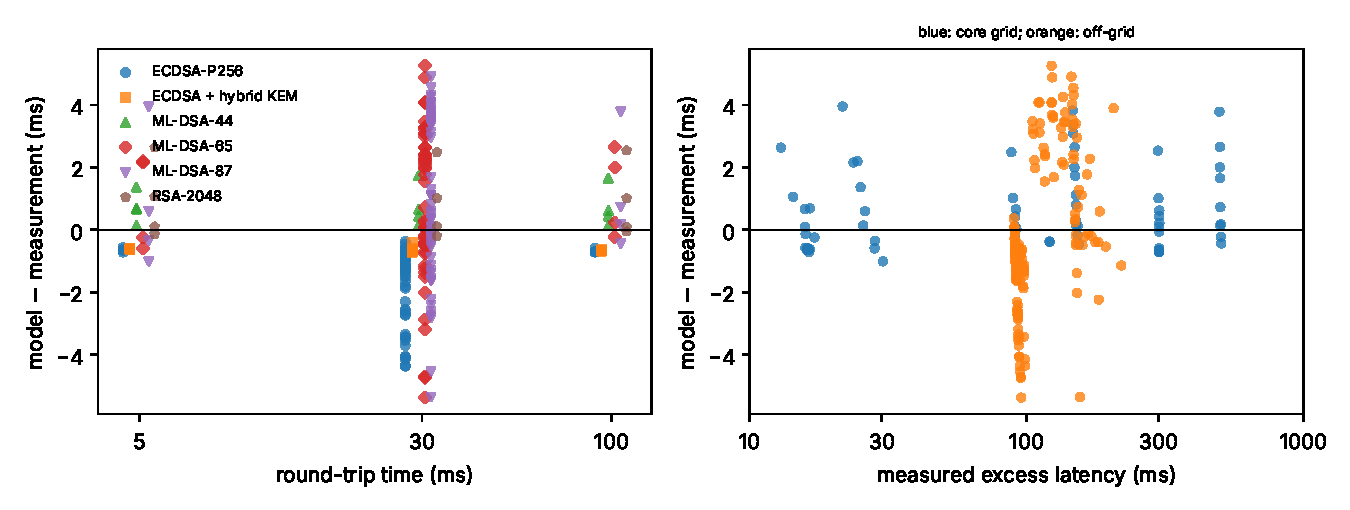
\includegraphics[width=\textwidth]{figures/fig_residuals}
\caption{Residuals of the stack model.}
\label{fig:residuals}
\end{figure}

In \cref{fig:residuals}, the left panel plots the residuals of the 82 core-grid and 144 off-grid configurations against the RTT by suite, and the right panel plots them against the measured excess latency. \Cref{tab:variants} evaluates the stack model under other TCP settings at 100\Mbits. Its columns give the MAE of the stack model and of the idealized model, the bias and maximum error of the stack model, the number of configurations above 0.4\,RTT (stack / idealized) and the difference $\Delta$ of measured excess latency against the Reno, quick-acknowledgment, no-timestamp run of the same configuration. CUBIC covers 5, 30 and 100\ms RTT, MTUs of 1\,280, 1\,500 and 9\,000\,bytes and initial windows of 10 and 32. The other rows use MTUs of 1\,280 and 1\,500\,bytes, an initial window of 10 and three suites. The model does not represent BBR; the BBR row marks the limit of the model.

\begin{table}[!htbp]\centering\small
\caption{Stack model under other TCP settings.}
\label{tab:variants}
\resizebox{\textwidth}{!}{\begin{tabular}{@{}lrrrrrrrrr@{}}
\toprule
Variant & $n$ & MAE (ms) & idealized MAE (ms) & bias (ms) & max (ms) & off $>0.4$ RTT (stack / idealized) & pairs & median $\Delta$ (ms) & max $|\Delta|$ (ms) \\
\midrule
CUBIC, quick ACK & 216 & 1.19 & 5.43 & +0.61 & 5.1 & 12 / 18 & 42 & +0.10 & 1.4 \\
Reno, delayed ACK & 72 & 1.26 & 11.04 & +0.48 & 3.8 & 5 / 11 & 42 & +0.14 & 0.7 \\
Reno, quick ACK, timestamps & 72 & 1.32 & 11.04 & +0.55 & 4.3 & 6 / 11 & 42 & +0.15 & 1.5 \\
Reno, delayed ACK, timestamps & 72 & 1.23 & 11.10 & +0.48 & 3.5 & 8 / 12 & 42 & +0.12 & 1.5 \\
BBR, quick ACK (exploratory) & 8 & 3.51 & 3.54 & -3.23 & 21.8 & 0 / 0 & 8 & +0.13 & 24.4 \\
\bottomrule
\end{tabular}}
\end{table}

\Cref{tab:status} records the standardization status of each scheme on 31 October 2026, read from csrc.nist.gov and datatracker.ietf.org on that date, and the measured components. TLS marks a run through a real TLS~1.3 handshake on the testbed. CPU marks a measured per-operation cost (\cref{tab:cpu,tab:cpux86}). Sizes marks certificate and signature sizes from real generated or published objects. Unmeasured quantities are modeled. Standardization status does not indicate deployment readiness, and the table does not assess library or HSM support.

\begin{table}[!htbp]\centering\footnotesize
\caption{Standardization status and measured components.}
\label{tab:status}
\resizebox{\textwidth}{!}{\begin{tabular}{@{}>{\raggedright\arraybackslash}p{0.15\textwidth}>{\raggedright\arraybackslash}p{0.17\textwidth}>{\raggedright\arraybackslash}p{0.17\textwidth}>{\raggedright\arraybackslash}p{0.22\textwidth}>{\raggedright\arraybackslash}p{0.05\textwidth}>{\raggedright\arraybackslash}p{0.05\textwidth}>{\raggedright\arraybackslash}p{0.06\textwidth}@{}}
\toprule
Scheme & NIST standard & X.509 profile (IETF) & TLS~1.3 specification & TLS & CPU & Sizes \\
\midrule
RSA-2048, ECDSA-P256 & FIPS 186-5 & RFC 5280 & RFC 9846 & yes & yes & yes \\
ML-KEM-768/1024; X25519\allowbreak{}MLKEM768 & FIPS 203 (13 Aug 2024) & -- & X25519\allowbreak{}MLKEM768: RFC 10024 (Aug 2026); pure ML-KEM groups: not assessed & yes & yes & yes \\
ML-DSA-44/65/87 & FIPS 204 (13 Aug 2024) & RFC 9881 (Oct 2025) & draft-ietf-tls-mldsa-06, RFC Editor queue, Informational & yes & yes & yes \\
SLH-DSA-128s/128f & FIPS 205 (13 Aug 2024) & RFC 9909 (Dec 2025) & no code points in OpenSSL~3.5 & no & yes & yes (certificates) \\
Falcon-512 (FN-DSA) & FIPS 206 in development (round-3 parameters used here) & draft-ietf-lamps-fn-dsa-certificates-00 (May 2026) & none & no & yes (liboqs) & sizes of the specification \\
Composite ML-DSA + ECDSA & -- & draft-ietf-lamps-pq-composite-sigs-19, RFC Editor queue & none & no & sum & sizes of the sum \\
\bottomrule
\end{tabular}}
\end{table}

\FloatBarrier

\section{Session tickets and server CPU}
\label{app:extra}
\Cref{tab:ticket} compares a full transaction that also issues a TLS~1.3 session ticket with the ticketless transaction of the main campaign. \Cref{tab:srvcpu} compares the CPU per transaction of an event-driven server with the primitive costs of the model.

\begin{table}[!htbp]\centering\small
\caption{A full transaction that also issues a session ticket against the ticketless one of the main campaign (excess latency over the unshaped run, ms; same suite, chain depth, RTT, MTU, initial window of 10, 100\Mbits, 302/222-byte transaction, Reno with quick acknowledgments). The model has no mode for a full handshake with a ticket. In 6 of the 40 configurations that have a ticketless reference, the transaction with a ticket was slower by half a round trip (median 0.51 RTT); the median difference over all is 0.6\ms.}
\label{tab:ticket}
\resizebox{\textwidth}{!}{\begin{tabular}{@{}lrrrrrr@{}}
\toprule
Suite & depth & MTU & \multicolumn{3}{c}{ticket minus no ticket (ms) at RTT} & in RTT \\
\cmidrule(lr){4-6}
 & & & 5\,ms & 30\,ms & 100\,ms & (30, 100\,ms) \\
\midrule
ECDSA-P256 & 1 & 1280 & -- & +0.2 & -- & +0.01 \\
ECDSA-P256 & 1 & 1500 & +0.2 & +0.3 & +0.4 & +0.01 \\
ECDSA-P256 & 3 & 1500 & +0.3 & +14.9 & +50.1 & +0.50 \\
ECDSA-P256 + hybrid KEM & 1 & 1280 & -- & +0.2 & -- & +0.01 \\
ECDSA-P256 + hybrid KEM & 1 & 1500 & +0.2 & +0.2 & +0.2 & +0.00 \\
ECDSA-P256 + hybrid KEM & 3 & 1500 & +0.3 & +0.3 & +0.4 & +0.01 \\
ML-DSA-44 & 1 & 1500 & +1.2 & +15.6 & +50.8 & +0.51 \\
ML-DSA-44 & 3 & 1500 & +0.8 & +0.9 & +0.9 & +0.02 \\
ML-DSA-65 & 1 & 1280 & -- & -0.1 & -- & -0.00 \\
ML-DSA-65 & 1 & 1500 & +0.5 & +15.8 & +50.8 & +0.52 \\
ML-DSA-65 & 3 & 1500 & +0.8 & +0.8 & +0.9 & +0.02 \\
ML-DSA-87 & 1 & 1280 & -- & +0.6 & -- & +0.02 \\
ML-DSA-87 & 1 & 1500 & +0.6 & +0.7 & +0.6 & +0.01 \\
ML-DSA-87 & 3 & 1500 & +0.9 & +0.9 & +1.0 & +0.02 \\
RSA-2048 & 1 & 1500 & +1.9 & +2.0 & +2.0 & +0.04 \\
RSA-2048 & 3 & 1500 & +0.3 & +0.2 & +0.3 & +0.00 \\
\bottomrule
\end{tabular}
}
\end{table}

\begin{table}[!htbp]\centering\small
\caption{CPU per transaction of an event-driven OpenSSL~3.5.4 server on one Cortex-X925 core (loopback, saturated by a multi-threaded load generator; user and system CPU of the server process over the measurement window divided by the transactions it completed; ms) against the sum of the primitive costs of the model for the same operations. Chain depth 2, or 1 for resumed.}
\label{tab:srvcpu}
\resizebox{\textwidth}{!}{\begin{tabular}{@{}lrrrrrrrrr@{}}
\toprule
Suite & \multicolumn{3}{c}{server auth, depth 2} & \multicolumn{3}{c}{mutual TLS, depth 2} & \multicolumn{3}{c}{resumed, mutual TLS} \\
\cmidrule(lr){2-4}\cmidrule(lr){5-7}\cmidrule(lr){8-10}
 & measured & primitives & ratio & measured & primitives & ratio & measured & primitives & ratio \\
\midrule
ECDSA-P256 & 0.137 & 0.050 & 2.7 & 0.323 & 0.174 & 1.9 & 0.182 & 0.036 & 5.0 \\
ECDSA-P256 + hybrid KEM & 0.165 & 0.060 & 2.8 & 0.350 & 0.183 & 1.9 & 0.211 & 0.045 & 4.7 \\
RSA-2048 & 0.631 & 0.533 & 1.2 & 0.739 & 0.578 & 1.3 & 0.193 & 0.043 & 4.5 \\
ML-DSA-44 & 0.480 & 0.369 & 1.3 & 0.755 & 0.573 & 1.3 & 0.175 & 0.009 & 19.1 \\
ML-DSA-65 & 0.722 & 0.595 & 1.2 & 1.105 & 0.904 & 1.2 & 0.182 & 0.009 & 19.8 \\
ML-DSA-87 & 0.838 & 0.681 & 1.2 & 1.399 & 1.157 & 1.2 & 0.198 & 0.012 & 16.7 \\
\bottomrule
\end{tabular}
}
\end{table}

%% References (generated with elsarticle-num and included here)
\begin{thebibliography}{10}
\expandafter\ifx\csname url\endcsname\relax
  \def\url#1{\texttt{#1}}\fi
\expandafter\ifx\csname urlprefix\endcsname\relax\def\urlprefix{URL }\fi
\expandafter\ifx\csname href\endcsname\relax
  \def\href#1#2{#2} \def\path#1{#1}\fi

\bibitem{fips204}
{National Institute of Standards and Technology}, Module-lattice-based digital
  signature standard, FIPS 204, U.S. Department of Commerce (2024).
\newblock \href {https://doi.org/10.6028/NIST.FIPS.204}
  {\path{doi:10.6028/NIST.FIPS.204}}.

\bibitem{shor1994}
P.~W. Shor, Algorithms for quantum computation: discrete logarithms and
  factoring, in: Proc. 35th Annual Symposium on Foundations of Computer Science
  (FOCS), IEEE, 1994, pp. 124--134.
\newblock \href {https://doi.org/10.1109/SFCS.1994.365700}
  {\path{doi:10.1109/SFCS.1994.365700}}.

\bibitem{mosca2018}
M.~Mosca, Cybersecurity in an era with quantum computers: will we be ready?,
  IEEE Security \& Privacy 16~(5) (2018) 38--41.
\newblock \href {https://doi.org/10.1109/MSP.2018.3761723}
  {\path{doi:10.1109/MSP.2018.3761723}}.

\bibitem{baradziej2026}
S.~Baradziej, Harvest now, decrypt later as a cross-sector threat: a scoping
  review of data-confidentiality lifetimes against post-quantum migration
  readiness, International Journal of Computational Intelligence
  Systems{P}ublished online 20 August 2026 (2026).
\newblock \href {https://doi.org/10.1007/s44196-026-01526-2}
  {\path{doi:10.1007/s44196-026-01526-2}}.

\bibitem{fips203}
{National Institute of Standards and Technology}, Module-lattice-based
  key-encapsulation mechanism standard, FIPS 203, U.S. Department of Commerce
  (2024).
\newblock \href {https://doi.org/10.6028/NIST.FIPS.203}
  {\path{doi:10.6028/NIST.FIPS.203}}.

\bibitem{fips205}
{National Institute of Standards and Technology}, Stateless hash-based digital
  signature standard, FIPS 205, U.S. Department of Commerce (2024).
\newblock \href {https://doi.org/10.6028/NIST.FIPS.205}
  {\path{doi:10.6028/NIST.FIPS.205}}.

\bibitem{baseri2024}
Y.~Baseri, V.~Chouhan, A.~Hafid, Navigating quantum security risks in networked
  environments: a comprehensive study of quantum-safe network protocols,
  Computers \& Security 142 (2024) 103883.
\newblock \href {https://doi.org/10.1016/j.cose.2024.103883}
  {\path{doi:10.1016/j.cose.2024.103883}}.

\bibitem{baseri2026}
Y.~Baseri, V.~Chouhan, A.~Ghorbani, Cybersecurity in the quantum era: assessing
  the impact of quantum computing on infrastructure, Computers \& Security 167
  (2026) 104917.

\bibitem{bis_leap2023}
{BIS Innovation Hub Eurosystem Centre, Banque de France, Deutsche Bundesbank},
  \href{https://www.bis.org/publ/othp67.pdf}{{Project Leap}, phase 1:
  Quantum-proofing the financial system}, Tech. rep., Bank for International
  Settlements (Jun. 2023).
\newline\urlprefix\url{https://www.bis.org/publ/othp67.pdf}

\bibitem{bis_leap2025}
{BIS Innovation Hub Eurosystem Centre and Banca d'Italia and Banque de France
  and Deutsche Bundesbank and Nexi-Colt and Swift},
  \href{https://www.bis.org/publications/project-leap-phase-2-quantum-proofing-payment-systems}{{Project
  Leap}, phase 2: Quantum-proofing payment systems}, Tech. rep., Bank for
  International Settlements (Dec. 2025).
\newline\urlprefix\url{https://www.bis.org/publications/project-leap-phase-2-quantum-proofing-payment-systems}

\bibitem{sikeridis2020}
D.~Sikeridis, P.~Kampanakis, M.~Devetsikiotis, Post-quantum authentication in
  {TLS} 1.3: a performance study, in: Proc. Network and Distributed System
  Security Symposium (NDSS), 2020.

\bibitem{paquin2020}
C.~Paquin, D.~Stebila, G.~Tamvada, Benchmarking post-quantum cryptography in
  {TLS}, in: Post-Quantum Cryptography (PQCrypto 2020), Vol. 12100 of Lecture
  Notes in Computer Science, Springer, 2020, pp. 72--91.

\bibitem{montenegro2026}
J.~A. Montenegro, R.~Rios, J.~Lopez-Cerezo, A performance evaluation framework
  for post-quantum {TLS}, Future Generation Computer Systems 175 (2026) 108062.
\newblock \href {https://doi.org/10.1016/j.future.2025.108062}
  {\path{doi:10.1016/j.future.2025.108062}}.

\bibitem{kampanakis2022}
P.~Kampanakis, M.~Kallitsis, Faster post-quantum {TLS} handshakes without
  intermediate {CA} certificates, in: Cyber Security, Cryptology, and Machine
  Learning (CSCML 2022), Vol. 13301 of Lecture Notes in Computer Science,
  Springer, 2022, pp. 337--355.
\newblock \href {https://doi.org/10.1007/978-3-031-07689-3_25}
  {\path{doi:10.1007/978-3-031-07689-3_25}}.

\bibitem{linuxtcp}
{Linux kernel developers}, {\texttt{tcp\_is\_cwnd\_limited()}} in
  \texttt{include/net/tcp.h}, linux kernel 6.14 (identical in 6.11), Source
  code, \url{https://github.com/torvalds/linux}, inspected in the installed
  headers of 6.11 and 6.14; the behavior of the testbed kernel (7.0) was
  measured (2025).

\bibitem{raavi2025}
M.~Raavi, Q.~Khan, S.~Wuthier, P.~Chandramouli, Y.~Balytskyi, S.-Y. Chang,
  Security and performance analyses of post-quantum digital signature
  algorithms and their {TLS} and {PKI} integrations, Cryptography 9~(2) (2025)
  38.
\newblock \href {https://doi.org/10.3390/cryptography9020038}
  {\path{doi:10.3390/cryptography9020038}}.

\bibitem{westerbaan2021}
B.~Westerbaan,
  \href{https://blog.cloudflare.com/sizing-up-post-quantum-signatures/}{Sizing
  up post-quantum signatures}, Cloudflare blog, 8 November 2021 (2021).
\newline\urlprefix\url{https://blog.cloudflare.com/sizing-up-post-quantum-signatures/}

\bibitem{bdfmas2024}
{Banque de France and Monetary Authority of Singapore}, Post-quantum
  cryptography report: securing digital communications between central banks,
  Tech. rep., Banque de France and Monetary Authority of Singapore (Nov. 2024).

\bibitem{sikeridis2020b}
D.~Sikeridis, P.~Kampanakis, M.~Devetsikiotis, Assessing the overhead of
  post-quantum cryptography in {TLS} 1.3 and {SSH}, in: Proc. 16th
  International Conference on Emerging Networking EXperiments and Technologies
  (CoNEXT), 2020, pp. 149--156.

\bibitem{schwabe2020}
P.~Schwabe, D.~Stebila, T.~Wiggers, Post-quantum {TLS} without handshake
  signatures, in: Proc. ACM Conference on Computer and Communications Security
  (CCS), ACM, 2020, pp. 1461--1480.

\bibitem{g7qtwg2026}
{G7 Central Bank Quantum Technologies Working Group}, Preparing for quantum
  technologies: key considerations for financial sector participants, Tech.
  rep., Banque de France and Bank of Canada (co-chairs) (May 2026).

\bibitem{andriani2024}
C.~Andriani, L.~Bencivelli, A.~Castellucci, M.~De~Santis, S.~Marchetti,
  G.~Piantanida, The quantum challenge: implications and strategies for a
  secure financial system, Questioni di Economia e Finanza (Occasional Papers)
  877, Banca d'Italia (Oct. 2024).

\bibitem{dora2022}
{European Parliament and Council of the European Union}, Regulation ({EU})
  2022/2554 on digital operational resilience for the financial sector
  ({DORA}), {O}fficial {J}ournal of the {E}uropean {U}nion (2022).

\bibitem{janciute2025}
L.~Jan{\v c}i{\=u}t{\.e}, Cybersecurity in the financial sector and the
  quantum-safe cryptography transition: in search of a precautionary approach
  in the {EU} {Digital Operational Resilience Act} framework, International
  Cybersecurity Law Review 6 (2025) 145--154.
\newblock \href {https://doi.org/10.1365/s43439-025-00135-7}
  {\path{doi:10.1365/s43439-025-00135-7}}.

\bibitem{falcon2020}
P.-A. Fouque, J.~Hoffstein, P.~Kirchner, V.~Lyubashevsky, T.~Pornin, T.~Prest,
  T.~Ricosset, G.~Seiler, W.~Whyte, Z.~Zhang, Falcon: fast-{Fourier}
  lattice-based compact signatures over {NTRU}, Specification submitted to the
  NIST Post-Quantum Cryptography project (round 3) (2020).

\bibitem{compositedraft}
M.~Ounsworth, J.~Gray, M.~Pala, J.~Klau{\ss}ner, S.~Fluhrer, Composite
  module-lattice-based digital signature algorithm ({ML-DSA}) for use in
  {X.509} public key infrastructure, Internet-Draft
  draft-ietf-lamps-pq-composite-sigs-19 (not yet an RFC: in the RFC Editor
  queue, final approval pending), {IETF}, accessed 31 October 2026 (2026).

\bibitem{hybriddraft}
K.~Kwiatkowski, P.~Kampanakis, B.~Westerbaan, D.~Stebila, Post-quantum
  traditional ({PQ/T}) hybrid key agreement mechanisms for {TLS} 1.3, {IETF}
  RFC 10024 (2026).

\bibitem{iso8583}
{International Organization for Standardization}, {ISO} 8583:2023, financial
  transaction card originated messages --- interchange message specifications
  (2023).

\bibitem{iso20022}
{International Organization for Standardization}, {ISO} 20022: financial
  services --- universal financial industry message scheme, ISO 20022 series
  (2013).

\bibitem{xmldsig}
D.~Eastlake, et~al., {XML} signature syntax and processing version 1.1, W3C
  Recommendation (2013).

\bibitem{rfc6749}
D.~Hardt, The {OAuth} 2.0 authorization framework, {IETF} RFC 6749 (2012).

\bibitem{rfc6750}
M.~Jones, D.~Hardt, The {OAuth} 2.0 authorization framework: bearer token
  usage, {IETF} RFC 6750 (2012).

\bibitem{oidccore}
N.~Sakimura, J.~Bradley, M.~Jones, B.~de~Medeiros, C.~Mortimore, {OpenID
  Connect} core 1.0 incorporating errata set 1, OpenID Foundation (2014).

\bibitem{fapi2}
{OpenID Foundation}, {FAPI} 2.0 security profile, Final specification (2025).

\bibitem{rfc9449}
D.~Fett, et~al., {OAuth} 2.0 demonstrating proof of possession ({DPoP}), {IETF}
  RFC 9449 (2023).

\bibitem{rfc8705}
B.~Campbell, et~al., {OAuth} 2.0 mutual-{TLS} client authentication and
  certificate-bound access tokens, {IETF} RFC 8705 (2020).

\bibitem{fips186}
{National Institute of Standards and Technology}, Digital signature standard
  (DSS), FIPS 186-5, U.S. Department of Commerce (2023).

\bibitem{sosnowski2023}
M.~Sosnowski, F.~Wiedner, E.~Hauser, L.~Steger, D.~Schoinianakis,
  S.~Gallenm{\"u}ller, G.~Carle, The performance of post-quantum {TLS}~1.3, in:
  Companion of the 19th International Conference on emerging Networking
  EXperiments and Technologies (CoNEXT Companion '23), ACM, 2023, pp. 19--27.
\newblock \href {https://doi.org/10.1145/3624354.3630585}
  {\path{doi:10.1145/3624354.3630585}}.

\bibitem{kampanakis2018}
P.~Kampanakis, P.~Panburana, E.~Daw, D.~Van~Geest, The viability of
  post-quantum {X.509} certificates, Cryptology ePrint Archive, Paper 2018/063
  (2018).
\newblock \url{https://eprint.iacr.org/2018/063}

\bibitem{burstinghaus2020}
K.~B{\"u}rstinghaus-Steinbach, C.~Krau{\ss}, R.~Niederhagen, M.~Schneider,
  Post-quantum {TLS} on embedded systems: integrating and evaluating {Kyber}
  and {SPHINCS+} with {mbed TLS}, in: Proc. ACM Asia Conference on Computer and
  Communications Security (AsiaCCS), 2020, pp. 841--852.
\newblock \href {https://doi.org/10.1145/3320269.3384725}
  {\path{doi:10.1145/3320269.3384725}}.

\bibitem{mtcdraft}
D.~Benjamin, D.~O'Brien, B.~Westerbaan, L.~Valenta, F.~Valsorda, Merkle tree
  certificates, Internet-Draft draft-ietf-plants-merkle-tree-certs-07 (work in
  progress), IETF (2026).

\bibitem{bdf2022}
{Banque de France}, Report on the ``post-quantum'' trial: post-quantum data
  exchange security solution, Technical report, Banque de France (November
  2022).

\bibitem{rfc5280}
D.~Cooper, et~al., Internet {X.509} public key infrastructure certificate and
  certificate revocation list ({CRL}) profile, {IETF} RFC 5280 (2008).

\bibitem{rfc8446}
E.~Rescorla, The {Transport Layer Security} ({TLS}) protocol version 1.3,
  {IETF} RFC 9846 (obsoletes RFC 8446) (2026).

\bibitem{rfc6928}
J.~Chu, N.~Dukkipati, Y.~Cheng, M.~Mathis, Increasing {TCP}'s initial window,
  {IETF} RFC 6928 (2013).

\bibitem{rfc5681}
M.~Allman, V.~Paxson, E.~Blanton, {TCP} congestion control, {IETF} RFC 5681
  (2009).

\bibitem{rfc7661}
G.~Fairhurst, A.~Sathiaseelan, R.~Secchi, Updating {TCP} to support
  rate-limited traffic, RFC 7661, IETF (2015).

\bibitem{rfc8879}
A.~Ghedini, V.~Vasiliev, {TLS} certificate compression, {IETF} RFC 8879 (2020).

\bibitem{openssl35}
{OpenSSL Project}, {OpenSSL} 3.5.4, \url{https://www.openssl.org}, released 30
  September 2025 (2025).

\bibitem{stebila2016}
D.~Stebila, M.~Mosca, Post-quantum key exchange for the {Internet} and the
  {Open Quantum Safe} project, in: Selected Areas in Cryptography (SAC 2016),
  Lecture Notes in Computer Science, Springer, 2016, pp. 14--37.

\bibitem{tlsmldsa}
T.~Hollebeek, S.~Schmieg, B.~Westerbaan, Use of {ML-DSA} in {TLS} 1.3,
  Internet-Draft draft-ietf-tls-mldsa-06 (not yet an RFC: in the RFC Editor
  queue, intended Informational), {IETF}, accessed 31 October 2026 (2026).

\bibitem{tlsmlkem}
D.~Connolly, {ML-KEM} post-quantum key agreement for {TLS} 1.3, Internet-Draft
  draft-ietf-tls-mlkem-11 (in the RFC Editor queue, intended Informational),
  {IETF}, accessed 2 November 2026 (2026).

\bibitem{rfc9438}
L.~Xu, S.~Ha, I.~Rhee, V.~Goel, L.~Eggert, {CUBIC} for fast and long-distance
  networks, {IETF} RFC 9438 (2023).

\bibitem{dinh2026artifact}
T.-H. Dinh, T.-M. Hoang, pqc-financial-transport: simulator, measurements and paper assets
  (software and data), Zenodo, version paper1-v1.3, all versions:
  10.5281/zenodo.23839449 (2026).
\newblock \href {https://doi.org/10.5281/zenodo.23839449}
  {\path{doi:10.5281/zenodo.23839449}}.

\end{thebibliography}
\end{document}
